\chapter{Cosmic Rays and Neutrinos}
\label{ch:cr}

\url{https://indico.cern.ch/event/719824/contributions/2972435/attachments/1745570/2825844/ISAPP2018_CERN_parizot.pdf} NALEZEN

Cosmic rays alsmost exclusively refer to particles with a finite rest mass. The term \textit{rays} was historically wrongly attributed to these particles as they were thought to be mostly electromagnetic radiation.
The interest of cosmic rays within the field of particle physics and modern particle physics is clear: multiple new particles were discovered from the interactions at energies which were higher than most experiments could reach. Positrons, muons, pions and kaons were first discovered in cosmic ray experiments in the 1930s and 40s. Today, high-energy cosmic ray interactions are still of interest as the highest energies of these particles go beyond what is feasible at the most powerful accelorators such as the LHC. Neutrinos are expected be produced toghether with cosmic rays near the source or close to Earth making neutrino astronomy a powerful and important part of modern day astronomy. In this chapter I will give BLA BLA BLA. For a more exhaustive description of cosmic rays I refer the reader to \cite{Gaisser:2016uoy}.

\section{Cosmic rays}
\subsection{Discovery of cosmic rays}
With the use of electrometers, Victor Hess performed multiple ground-breaking balloon flight experiments in 1912 to prove that the amount of radiation increases with altitude \cite{hessnobel:1936}. This was in strong contradiction with the widespread belief that radiation on Earth's surface mostly originates from radioactive substances in its crust. Hess concluded that an extremely penetrating radiation existed. He described this radiation to be coming from space wich then enters Earth's atmosphere which proved to be correct but it was wrongfully attributed to electromagnetic radiation by Robert Millikan in the 1920s \cite{PhysRev.32.533}. 

Hess later ruled out the possibility that cosmic rays originate from the Sun as his observations showed no particular differences in night and day and during solar eclipses. In the late 1920s, first evidence was found that cosmic rays were charged due to a variation of their intensity with latitude \cite{clay:1927a}. This indicated that they were deflected by the geomagnetic field.

\subsection{What are cosmic rays?}
\label{subsec:whatarecosmicrays}
Cosmic rays are, almost exclusively, the collection of nuclei which are stripped of their electrons, making them electrically charged, heavy particles. Around 90\% of the particles are ionized hydrogen atoms, or protons. 9\% are alpha particles and 1\% are nuclei of heavier elements. There is a striking resemblance between the relative abundance of cosmic rays and elements in the Solar System as seen in Figure \ref{fig:relabundance}. A much smaller fraction of incoming particles are electrons, positron and antiprotons.

\begin{figure}
\centering
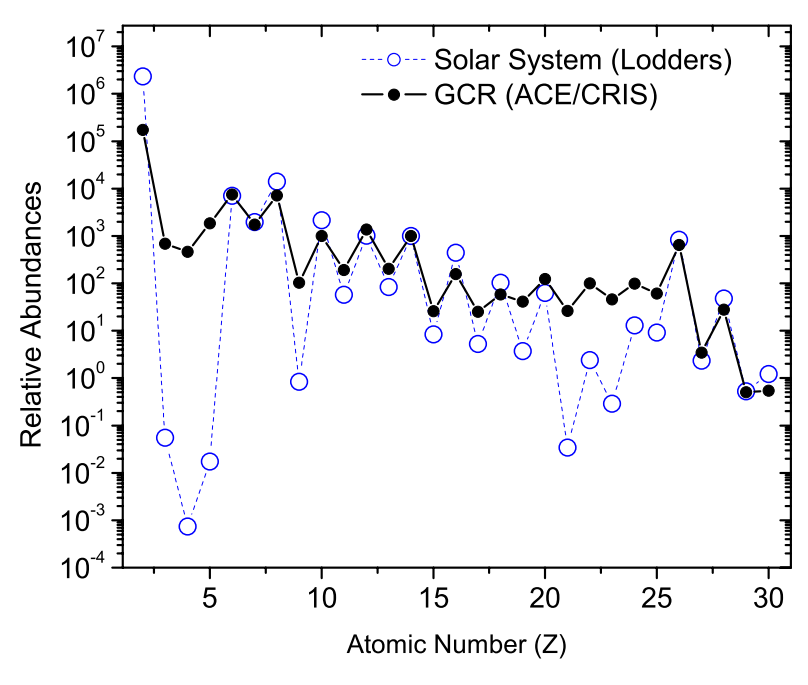
\includegraphics[width=0.7\textwidth]{./chapter3/img/relativeabundanceACE.png}
\caption{The cosmic ray elemental abundances measured on Earth compared to the solar system abundances, all relative to carbon = 100. Figure from ACE news archive \cite{ISRAEL2005201}.}
\label{fig:relabundance}
\end{figure}
There are however two important differences between cosmic rays and elements from our Solar System. Firstly, the two groups of elements Li, Be, B and Sc, Ti, V, Cr, Mn are many orders of magnitude more abundant in cosmic rays than in the solar system. This is due to their absence in stellar nucleosynthesis and are therefore not expected to be produced in large numbers. More massive cosmic rays (mainly C, O and Fe) can produce these nuclei in the process of \textit{spallation}. They are produced by collisions of cosmic rays with the interstellar medium. Therefore, these nuclei are sometimes referred to as \textit{secondary nuclei}.
The second difference is that nuclei with $Z>1$ are much more abundant with respect to hydrogen for cosmic rays. This phenomenon is not yet well understood but could be attributed to the difficulty to ionize hydrogen, necessary for acceleration processes.

The amount of cosmic rays seen on Earth is expressed in units of $\left[m^{-2} s^{-1} sr^{-1}\right]$. We can see in Figure \ref{fig:spectrumCR} that the cosmic ray flux follows a energy power law spectrum:

\begin{equation}
\label{eq:spectrum}
dNdE \varpropto E^{-\gamma} dE,
\end{equation} 
where $\gamma$ is called the \textit{spectrum index}. Because of the steepness of the spectrum it is often multiplied by a higher power of energy\footnote{The broad range in both energy and flux should convince the reader that many types of detectors are necessary to study the behaviour of cosmic rays. Low-energy particles are abundant and high-energy particles are much more rare. Both the energy and the incoming flux will determine the type and size of the detector.}.

\begin{figure}
\centering
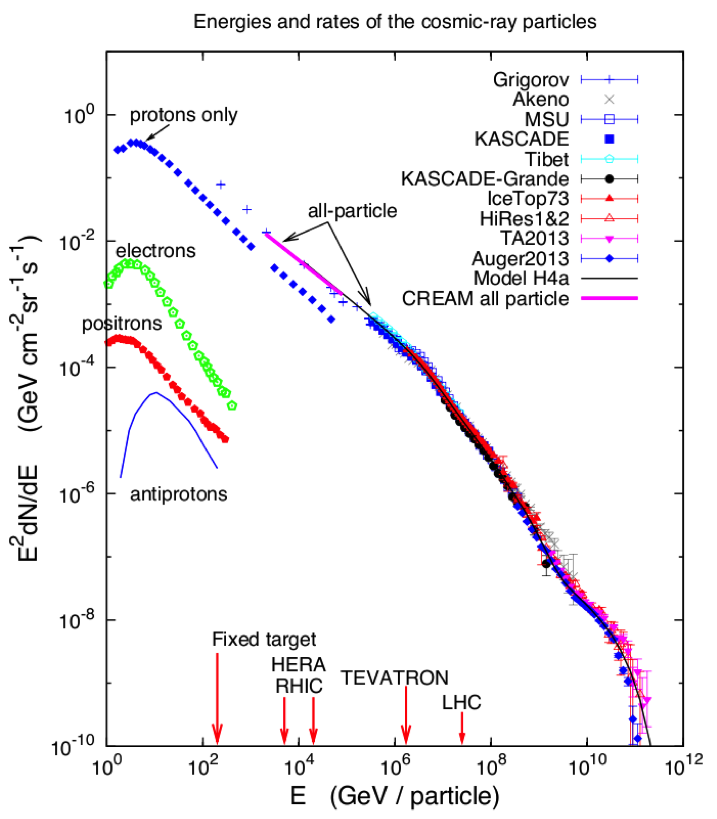
\includegraphics[width = 0.6\textwidth]{chapter3/img/spectrumCR.png}
\caption{Spectrum of cosmic rays at Earth. The all-particle spectrum measured by different experiments is plotted together with the proton-only spectrum. Subdominant contributions to the total flux from electrons, positrons and antiprotons as measured by the PAMELA experiment are also shown. Figure from \cite{Blasi:2013rva}.}
\label{fig:spectrumCR}
\end{figure}

We can divide the global spectrum in four regions. Between 10 GeV and 1 PeV the differential spectrum index is around -2.7. From 10 PeV to 1 EeV it is around -3.1. Above 10 EeV the spectrum again flattens to an index around -2.6 and an apparent cutoff region is present at around $10^{20}$ eV. The transition of this first to second region is referred to as the \textit{knee} at around 3 PeV. The second to third region transition is referred to as the \textit{ankle}. It is possible to describe the full cosmic-ray spectrum with sources within our galaxy. A more generally accepted theory is that the knee in the spectrum originates from the end of a population of particles which are accelerated within our Milky Way \cite{Gaisser:2013bla}. A sometimes referred to at around 100 PeV is the \textit{second knee}, believed to be a feature of the iron drop-off.
The origin of cosmic rays has been a topic of discussion for many years. We know now that most particles originate from sources in the local galaxy, having spent on average $10^7$ years in diffusive motion in the interstellar medium \cite{Gaisser:2013bla}. This is consistent with the resemblance of the relative abundances of cosmic rays and elements from our Solar System. However, there is no general consensus about the origin of the cosmic rays with energies above $3 \times 10^{18}$ eV. In the following, the abovementioned energy regions are discussed in more detail.

\subsubsection{Solar modulation}
In the Solar System a stream of charged particles is released from the Sun. This stream is mostly made up of electrons, protons and alpha particles with kinetic energies ranging between 0.5 and 10 keV. Within this solar wind plasma there is a magnetic field. Cosmic rays coming in to the Solar System interact with these particles and magnetic field. The influence is greatest on particles with the lowest charges. This effect is called \textit{solar modulation}. In effect, we see a strong suppression of cosmic rays at energies of 10 GeV and below.

\subsubsection{Galactic component}
The most probable acceleration mechanism for cosmic rays originating from our Galaxy is by shocks driven by expanding supernova remnants \cite{0034-4885-64-4-201}. From the ratio of primary to secondary nuclei it can be inferred that cosmic rays travel distances thousands of times greater than the thickness of the disk of the Galaxy. There is also an apparent decrease in the amount of matter that is traversed by cosmic rays with higher energies than with lower. Higher-energy cosmic rays seem to spend less time in the Galaxy than lower-energy ones and suggests that cosmic rays are accelerated before most propagation occurs \cite{Gaisser:2016uoy}.

The way the spectrum is fit is not set in stone. Here I will use the convention used by Gaisser, Stanev and Tilav described used in reference \cite{Gaisser:2013bla}. The spectrum is subdivided in three populations. The first population corresponds to the particles accelerated by supernova remnants, with the knee signaling the cutoff of this population. The second population is a higher-energy galactic component of unknown origin. The third generation will be described in more detail in \ref{subsec:ankle}. Assuming that the primary spectrum depends on the \textit{magnetic rigidity}\footnote{An assumption which is experimentally favored over other assumptions. Rigidity is an appropriate variable for interpreting changes in the spectrum due to propagation and acceleration in magnetic fields.},

\begin{equation}
R = \frac{pc}{Ze},
\end{equation}
where $Ze$ is the charge of a nucleus of total energy $E_{tot} = pc$ and relates to the gyroradius of a particle in a given magnetic field $B$ as

\begin{equation}
\label{eq:gyro}
r_L = \frac{R}{B}.
\end{equation}
If there is a characteristic regidity, $R_e$ above which a particular acceleration process reaches a limit, then the feature will show up in total energy first for protons, then for helium and so forth for heavier nuclei according to

\begin{equation}
E_{tot} = Ze \times R_e.
\end{equation}
This effect is visualised in Figure \ref{fig:fitsgaisser} and indicates that as one population reaches its maximum the composition becomes heavier. The second knee, reported by KASCADE-Grande \cite{Apel:2011mi} and GAMMA \cite{Garyaka:2008gs} could be explained with an ``iron knee'' bump.

\begin{figure}
\centering
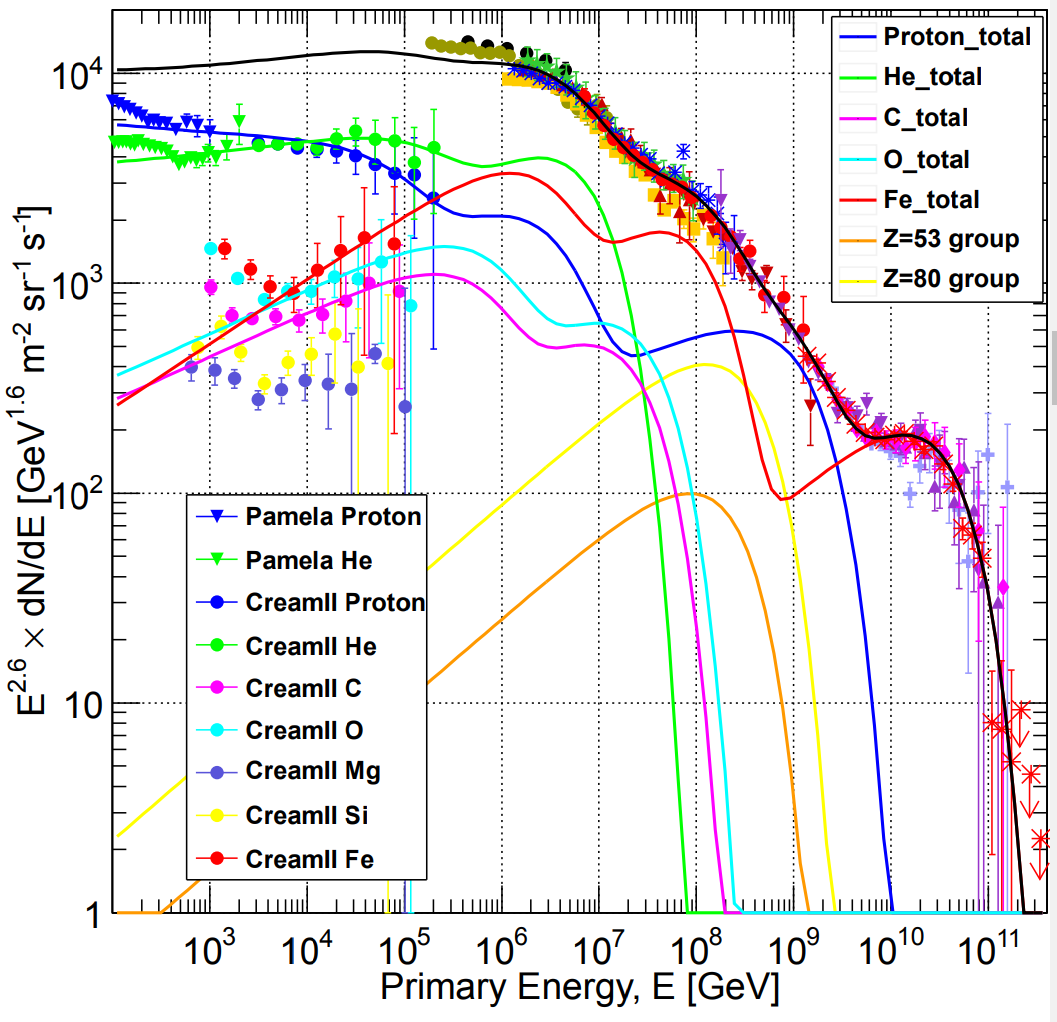
\includegraphics[width=0.48\textwidth]{chapter3/img/fit1gaisser.png}
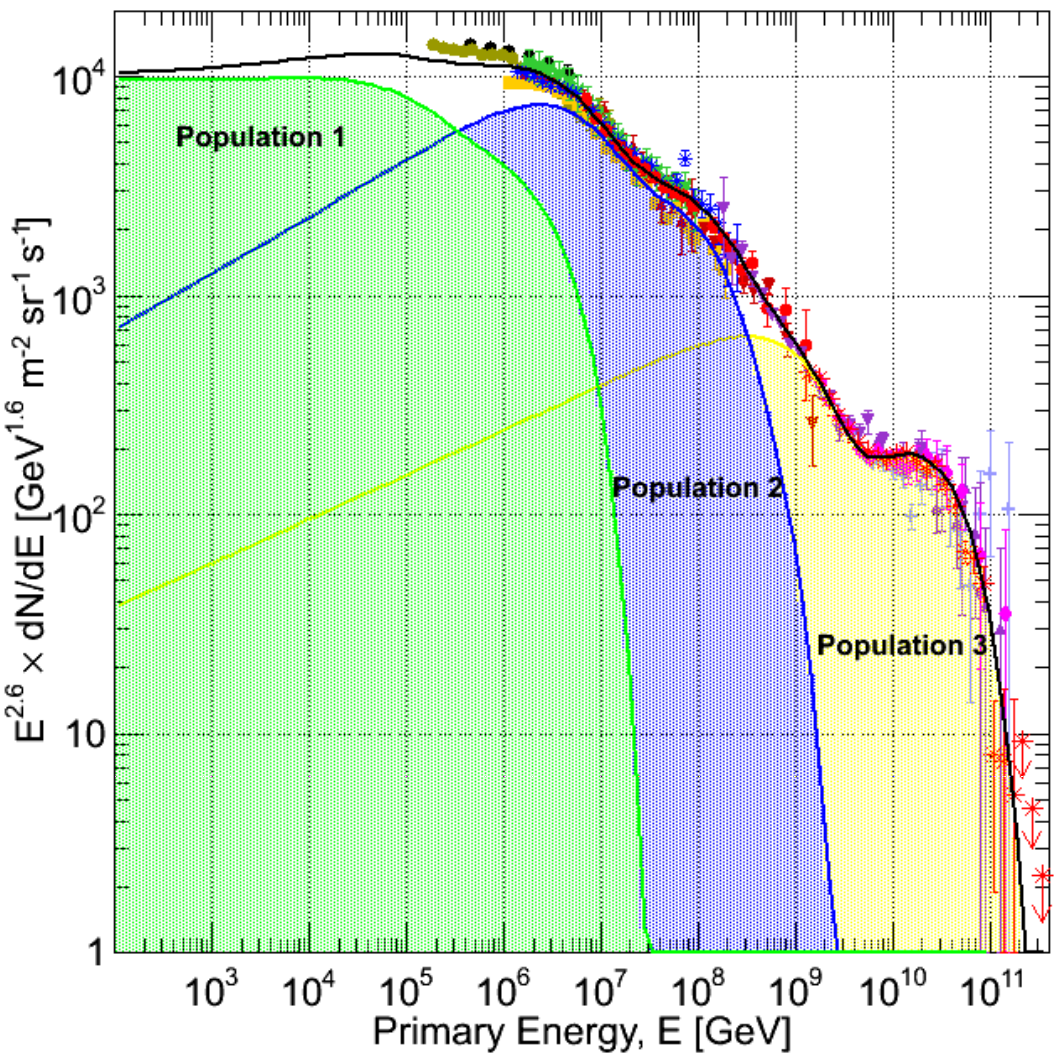
\includegraphics[width=0.48\textwidth]{chapter3/img/fit2gaisser.png}
\caption{Blub}
\label{fig:fitsgaisser}
\end{figure}

%A schematic picture of our home galaxy, the Milky Way, is shown in Fig. 1.2. Most stars are concentrated in the galactic disc of height h $\approx$ 300 pc in the form of spiral arms. The disc is filled with warm atomic gas that consists to 90\% of H and to 10\% of He and has an average density n approx 1/cm3. It contains also an ordered magnetic field with strength B approx 3microG. The energy when the Larmor radius
\subsubsection{Extragalactic component}
The flux at the highest energies is exceedingly small. The number of events per year at energies above $5 \times 10^{19}$ eV is around one per square kilometer per century. There are only two experiments in the world capable of detecting the highest-energy cosmic rays in a statistical meaningful way: Telescope Array, located in the Northern Hemisphere (area of $\approx$700 km$^2$) and the Pierre Auger Observatory in the Southern Hemisphere (area of $\approx$3000 km$^2$).

Both experiments see a suppression of the flux above $6 \times 10^{19}$ eV. The exponential cutoff is consistent with the expected Greisen-Zatsepin-Kuzmin (GZK) effect \cite{Greisen:1966jv,Zatsepin:1966jv} where cosmic rays interact with the cosmic microwave background radiation (CMB)

\begin{equation}
\gamma_{CMB} + p \rightarrow \Delta^+ \rightarrow p + \pi^0
\end{equation} 
or

\begin{equation}
\gamma_{CMB} + p \rightarrow \Delta^+ \rightarrow n + \pi^+.
\end{equation}
Particles with energies above $5 \times 10^{19}$ eV would interact with the CMB, leading to an exponential cutoff (but if the incoming particles above these energies would be relatively young it is still possible for them to reach the detector). The Pierre Auger experiment reported to see higher compositions at the highest energies \cite{icrc2017:pa}. If the particle is a nucleus with A nucleons, then the GZK limit applies to its nucleons, which carry only a fraction 1/A of the total energy. For iron nuclei this would for example result in a limit of $2.8 \times 10^{21}$ eV. In contrast, the TA experiment interpreted their data as implying a light primary composition (mainly p and He) at the highest energies. Both experiments use a different interpretations for crucial quantities of these measurements and a thorough join analysis conducted by both experiments states that, at the current level of statistics and understanding of systematics, both data sets are compatible with being drawn from the same parent distribution \cite{PDG2018url}.

\begin{figure}
\centering
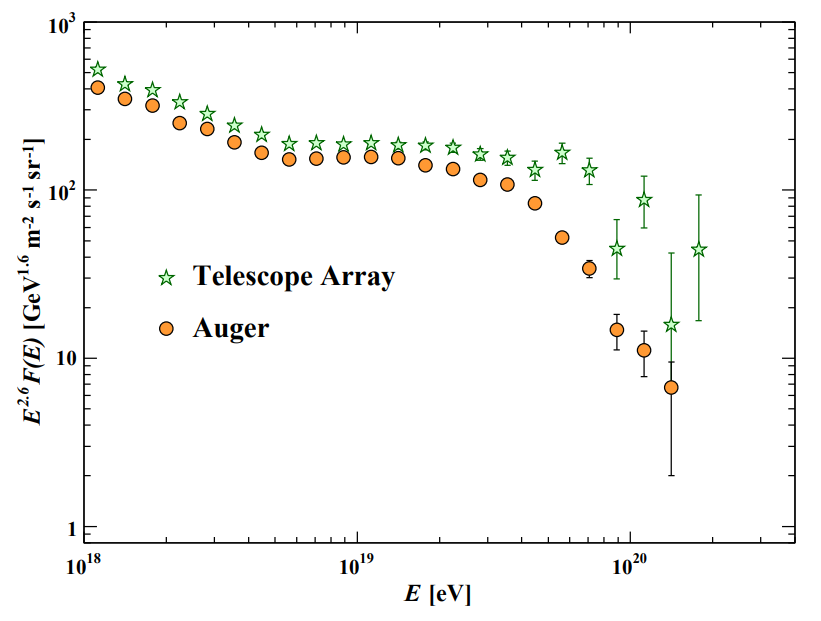
\includegraphics[width=0.6\textwidth]{chapter3/img/ankle.png}
\caption{Expanded view of the higest energy portion of the cosmic-ray spectrum from data of the Telescope Array and the Pierre Auger Observatory \cite{pdg2018}.}
\label{fig:ankle}
\end{figure}
The Pierre Auger Observatory also reported evidence in an anisotripic distribution of the arrival directions of the highest-energy cosmic rays \cite{Aab:2017tyv} in a direction where the distribution of galaxies is relatively high and does not coincide with the galactic plane. These observations, together with our lack of known possible sources within our galaxy for these ultra-high energies shows compelling evidence that these particles have an origin from outside our galaxy. From pion decay there is also an expected flux from extragalactic neutrinos (more information in section \ref{subsec:astro} and \ref{waarjehetinhoofdstuk5gaatbespreken}). The flux, spectrum and angular distribution of the excess neutrino signal detected by IceCube between $\approx 50$ TeV and $\approx 2$ PeV are inconsistent with those expected for Galactic sources \cite{Waxman:2013zda}.\\
\newline
To put it simply, understanding cosmic rays and where they originate can help us answer fundamental questions about the origins of the universe, our galaxy and ourselves. To put it in the words of Carl Sagan:

\begin{center}
\begin{minipage}[5cm]{0.9\textwidth}
\textit{``The nitrogen in our DNA, the calcium in our teeth, the iron in our blood, the carbon in our apple pies were made in the interiors of collapsing stars. We are made of starstuff.''}
\end{minipage}
\end{center}

\subsection{Acceleration mechanism}
How cosmic rays got their signature slope in the energy spectrum and its intricate details have been under discussion for multiple decades. To this date there is no clear picture how these particles are accelerated in full detail. It is beyond the scope of this work to give a comprehensive overview of all possible acceleration mechanisms or possible sources. Most calculations are left out and for a more detailed discussion the reader is referred to specialized books or the references in the text.\\
\newline
The acceleration of the particles can be subdivided into two questions. First, where are the particles accelerated? Does it happen on large scales, cosmological distances in galaxies or near specific sources? Secondly, how are these particles exactly accelerated? What is the driving mechanism? Since primary cosmic rays are all electromagnetically charged particles these mechanisms should clearly be sought for in places where electric and/or magnetic fields play a dominant role.

\subsubsection{Galactic accelerators}
With their approximate energy density around 0.5 eV/cm$^3$ in our local galaxy, the bulk of cosmic ray acceleration could very well be explained by \textbf{supernovae}. This density results into a total power of around

\begin{equation}
L_{CR} = 7 \times 10^{40} \textrm{ erg/s},
\end{equation}
where erg is a unit often used in astonomy\footnote{1 erg = $10^{-7}$ J.}. If one assumes a supernova explosion of around one per every 30 years then the total power output of type II supernovae with a mass output of around ten times the mass of the Sun at a velocity close to $5 \times 10^{8}$ cm/s would result in a power of

\begin{equation}
L_{SN} \backsim 3 \times 10^{42} \textrm{ erg/s}.
\end{equation}
These numbers are not set in stone and hold large uncertainties, but it shows that with an acceleration efficiency on the order of a couple of percent supernova explosions are a prominent source of energetic cosmic rays, if not the dominant one.

\subsubsection{Extragalactic accelerators}
We will see in Section \ref{para:maxenergy} that the maximum energy from shock acceleration by a supernova remnant is insufficient to explain UHECR. As explained in Section \ref{para:fermiacceleration}, particles can be accelerated if the trajectory of the particles can be changed and energy can be transferred multiple times. The magnetic fields responsible for the course change of these particles has to be sufficient in magnitude in order for these particles not to escape and go beyond the grasp of the source responsible for the acceleration. This limitation is expressed by the gyroradius in the accelerator, $r_L = E/ZeB$ similar to Eq. \ref{eq:gyro}, requiring it to be smaller than the radius of the accelerator: $r_L < R$ or $E < ZeBR$.

Even if only qualitative, this relation provides an interesting criterion to idendify possible sources of UHECRs by looking at the accelerator related term $BR$. This was done in a classic paper by Hillas \cite{Hillas:1985is}, illustrated in the more recent Figure \ref{fig:hillas}. Accelerators necessary to explain the amount of UHECRs are not populated (enough) in our galaxy, making them more likely to be of extra-galactic origin. \textbf{Active galactic nuclei, blazars and gamma ray bursts} (en andere als je die hebt toegevoegd later) are therefore also briefly explained.

\begin{figure}
\centering
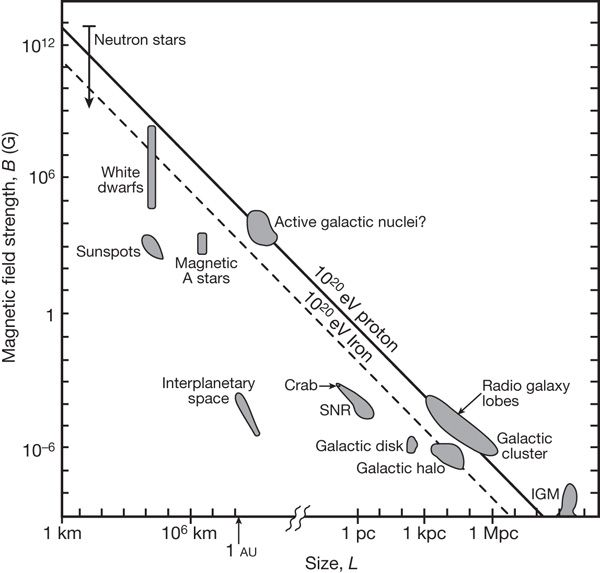
\includegraphics[width = 0.7\textwidth]{chapter3/img/Hillas.jpg}
\caption{The Hillas plot of potential cosmic ray accelerotors locates objects according to size and magnetic field. Objects to the left of the diagonal lines cannot accelerate particles to $10^{20}$ eV (proton: solid, iron: broken). Image obtained from HIER "REF" TOEVOEGEN, OVERAL EIGENLIJK \cite{Bauleo:2009zz}}
\label{fig:hillas}
\end{figure}



\subsection{Sources}
\subsubsection{Supernova (remnants)}
Supernovae can be broadly subdivided into two categories: type I and type II. Type I supernova explosions happen in binary star systems. In those systems one of the two starts is a carbon-oxygen white dwarf which accretes matter from the second star. When the total mass of the white dwarf reaches the Chandrasekhar REF limit of around 1.44 solar masses it cannot longer hold itself under the gravitational pressure and collapses in on itself. Within seconds, the carbon component in the white dwarf starts nuclear fusion and enough energy is released to produce an explosion brighter than the Sun with a factor of around 5 billion. 
A resulting shock wave can reach up to around 3\% the speed of light.

Type II supernova explosions differ by being single star systems. When a star reaches the end of its lifecycle the subsequent fusion reactions reach to a halt. If the star has enough mass (at least 8 times the mass of the Sun), it is possible for the inner core to again reach the Chandrasekhar limit and collapse in on itself due to the lack of \textit{electron degeneracy}. Without the outward pressure of nuclear fusion reactions and the support of the core, the outer layers of the star collapse under the gravitational pressure. The compression of the electrons and protons into neutrons results into a very hot, dense, neutron core. The velocity of the inwards falling layers can reach to a staggering 23\% of the speed of light and recoil when hitting the remaining core. Neutrinos are produced in this violent core collapse and the outward going shockwave hits the remaining outer layers forming the supernova explosion \footnote{Astronomer Carl Sagan once said, "The nitrogen in our DNA, the calcium in our teeth, the iron in our blood, the carbon in our apple pies were made in the interiors of collapsing stars. We are made of starstuff."}\footnote{To get a better feeling of how extraordinary these events really are, I'd like to illustrate what it would be when one could be close to a supernova event. From Figure \ref{fig:neutrinospectrumall} one can calculate that the number of of Solar neutrinos going through our hand per second is around \textit{one trillion}. Yet they are so weakly interaction, on average, only one will hit with an atom in your body every few years. Supernova explosions are so vast that around $10^{57}$ neutrinos can be released. This number is so big that even if an observer is a distance of 2.3 AU away from the event, he would still receive a fatal radiation dose of \textit{neutrinos alone}. As another example: looking at a supernova as far away as the Sun is from the Earth is $10^9$ times brighter than if one would detonate a hydrogen bomb pressed against your eyeball.}

Because of their brightness supernovae within our galaxy can be seen with the naked eye (provided they are not too far away). The last recorded supernova from our galaxy was by Johannes Kepler in 1604 but earliest recordings go back to 185 AD by Chinese astronomers\footnote{From observations of other galaxies supernovae are expected to occur, on average, once every thirty years. Not all of these will be visible to the naked eye, but would almost certainly be observable with modern astronomical telescopes.}.
\begin{figure}
\centering
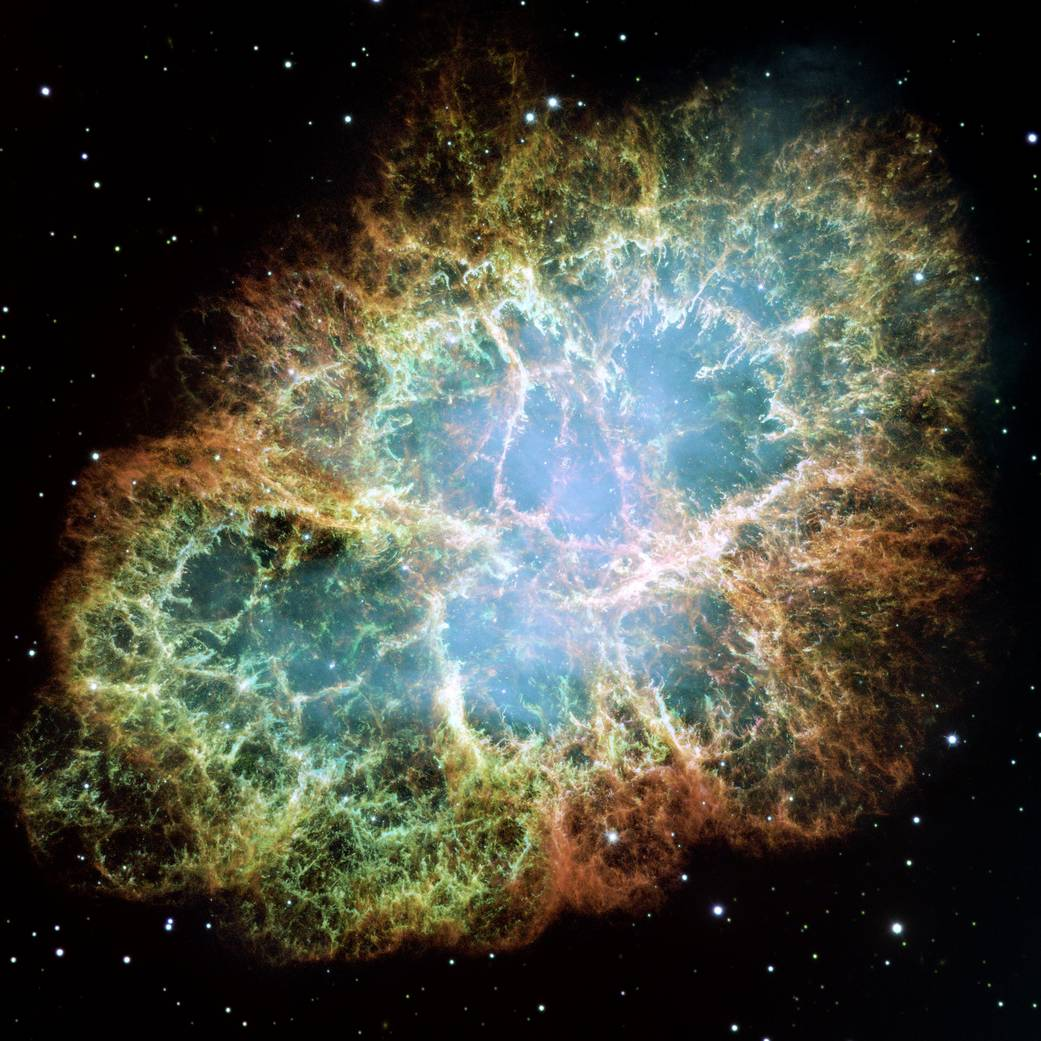
\includegraphics[width=0.48\textwidth,height=8cm]{chapter3/img/crabnebula.jpg}
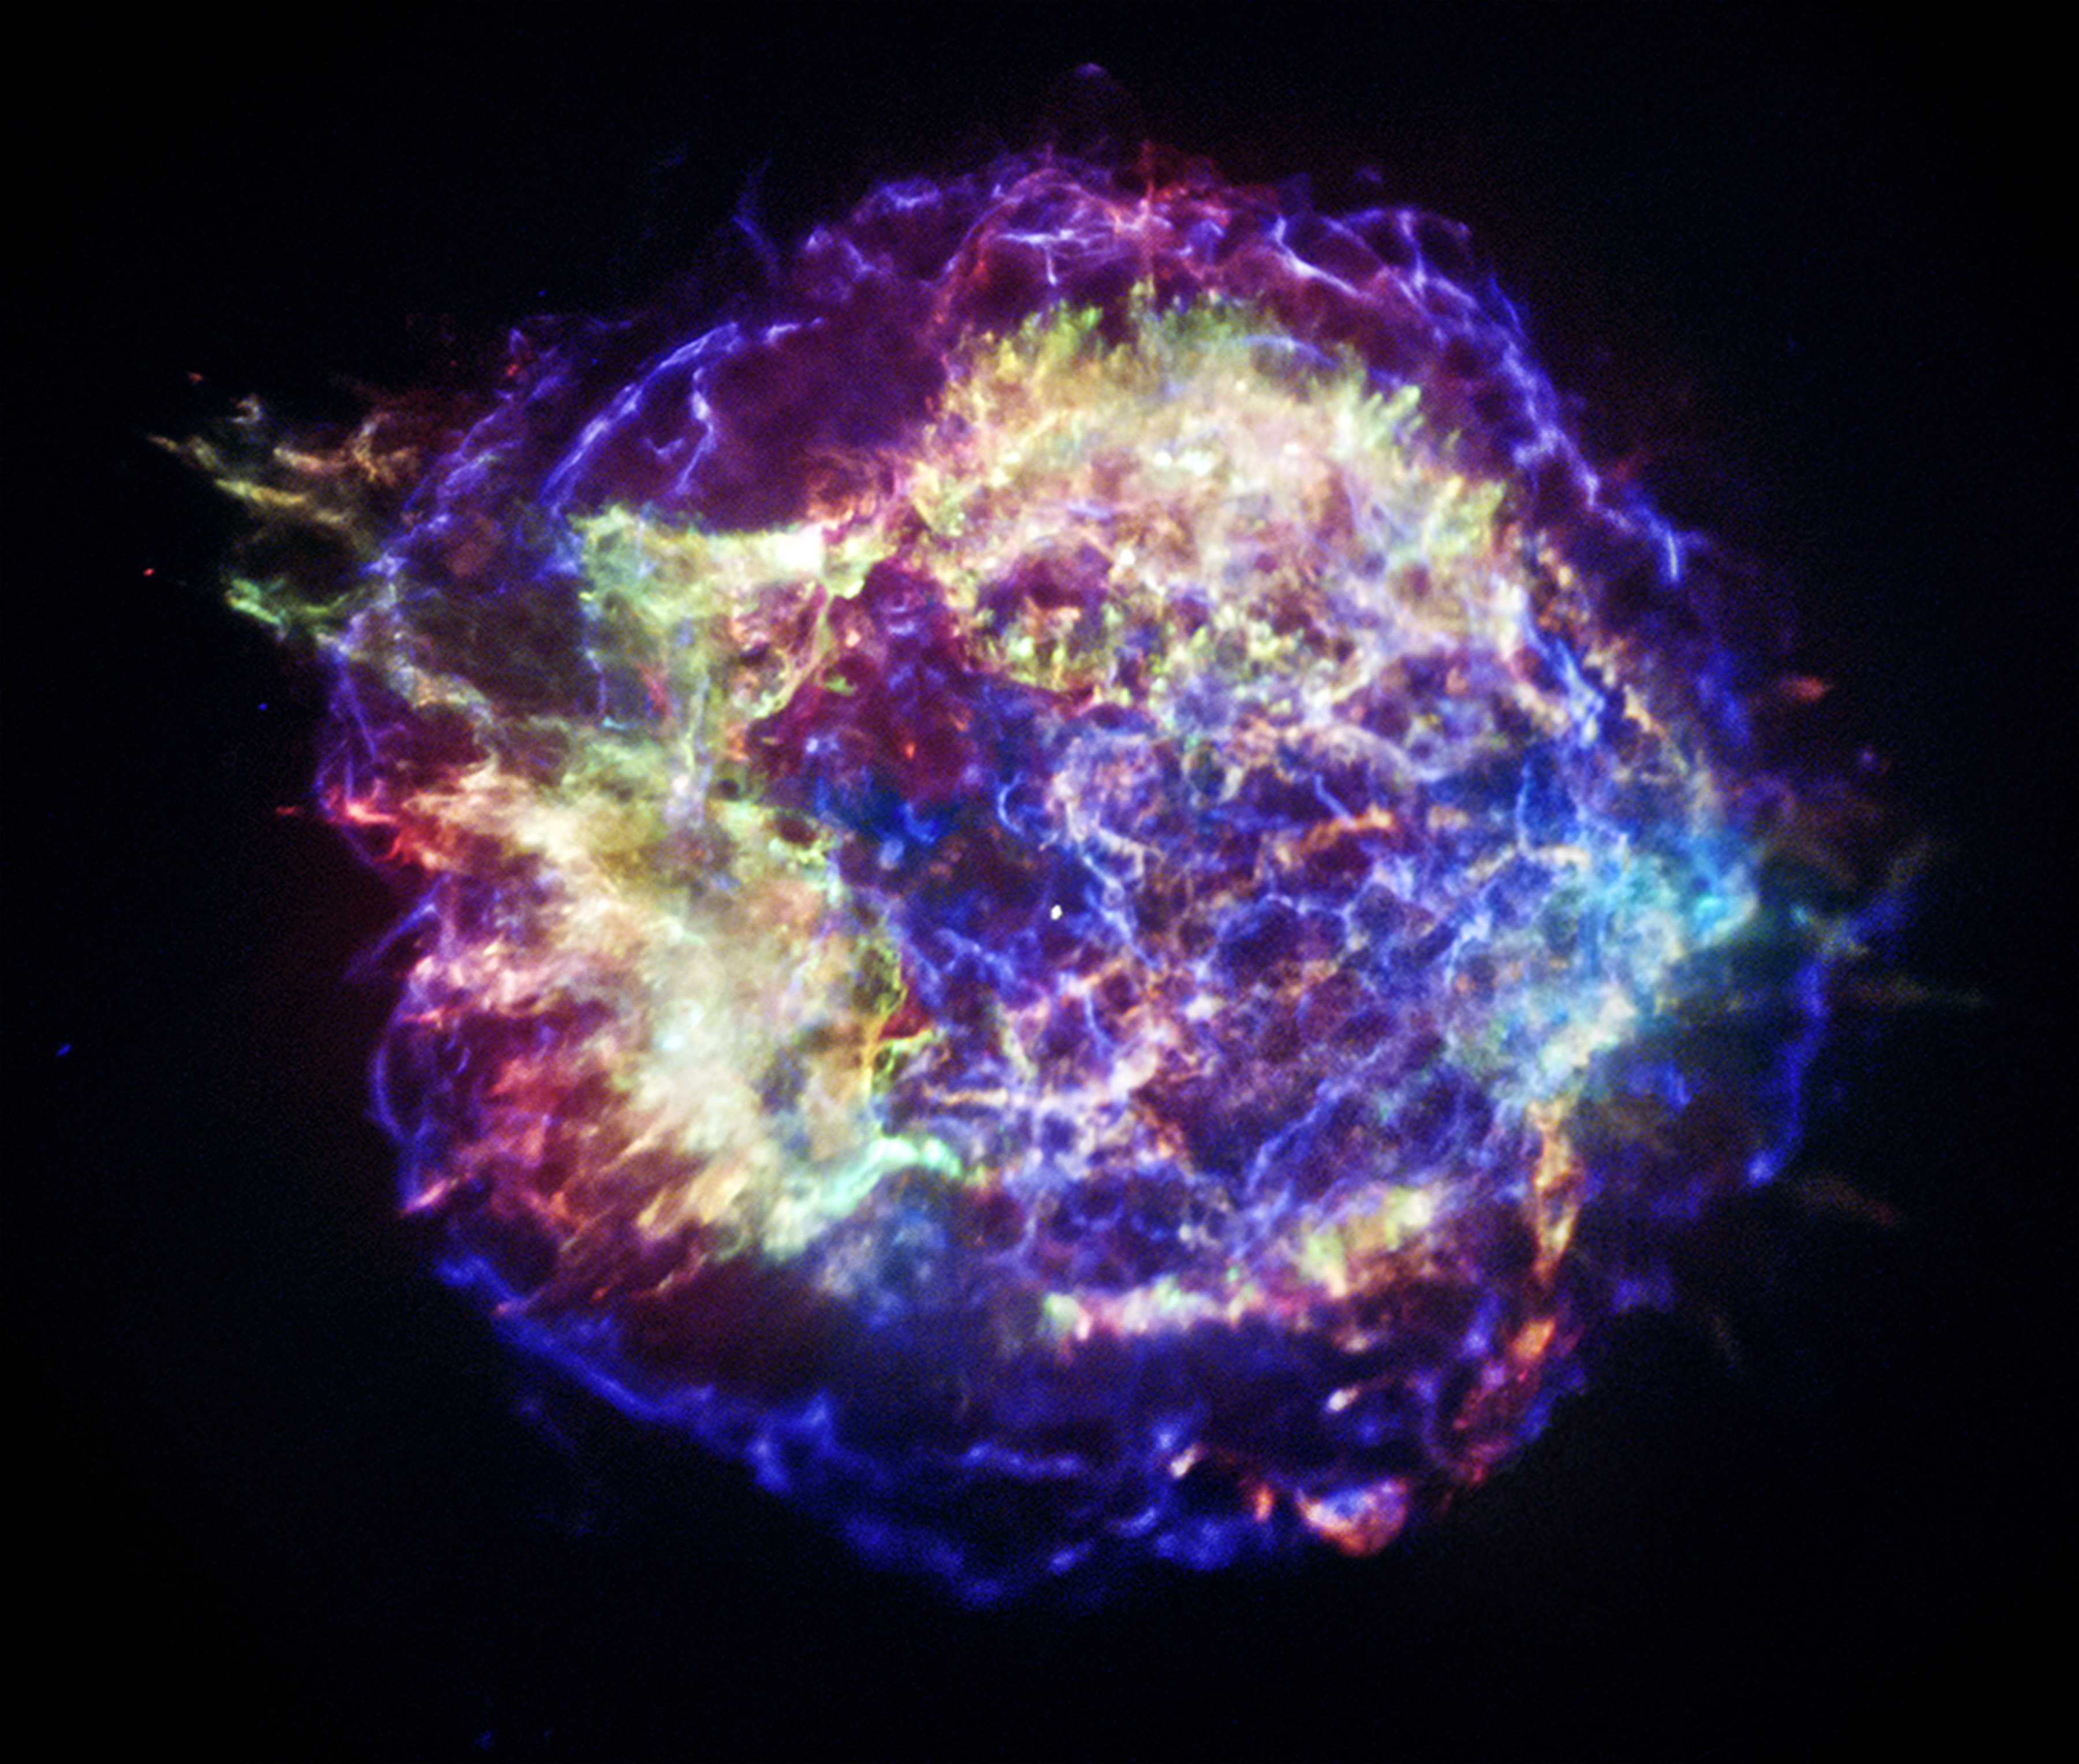
\includegraphics[width=0.48\textwidth,height=8cm]{chapter3/img/casa.jpg}
\caption{Left: the Crab Nebula is the supernova remnant approximately one thousand years old. The supernova was noted by Chinese astronomers in the year 1054 AD. Right: Chandra X-ray observatory picture of the Cassiopeia A supernova remnant (pictures from NASA).}
\label{fig:supernova}
\end{figure}
\newline
The question remains how supernovae can serve as cosmic ray accelerators. In 1949, Enrico fermi proposed a mechanism where particles can gain energy by collisions with moving interstellar ionized gas clouds. Only later, it was realized that a large, plane shock front moving with a certain velocity is able to accelerated charged particles much more efficiently. This first mechanism results into an energy transfer proportional to the squared velocity of the cloud and is thus called \textit{second order Fermi acceleration}. Shock front acceleration energy transfer is proportional to the velocity and is called \textit{first order Fermi acceleration}. Supernova remnants provide an explanation for the origin of these shock fronts.

\paragraph{First- and second-order Fermi acceleration}
\label{para:fermiacceleration}

Suppose we have a magnetic cloud in the interstellar medium travelling with a certain velocity $\vec{V}$ and a particle with velocity $\vec{v}$ enters the cloud under an angle $\theta_1$ (see Figure \ref{fig:cloud}). If we assume collisionless scattering can occur (no energy is dissipated from the particle to the cloud) due to the magnetic fields in the cloud, the magnitude of the momentum in the rest frame of the cloud will not change ($E'_1 = E'_2$, where we the apostrophe denotes the cloud rest frame). From special relativity we know that:

\begin{figure}
\centering
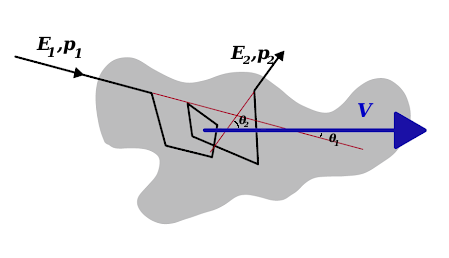
\includegraphics[width=0.48\textwidth]{chapter3/img/cloud.png}
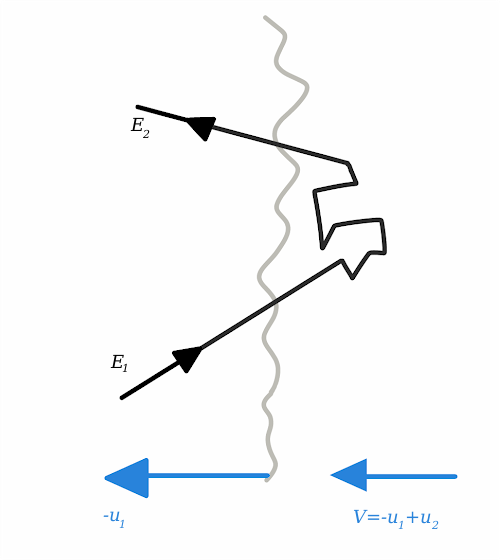
\includegraphics[width=0.48\textwidth]{chapter3/img/shock.png}
\caption{Left: magnetic cloud. Right: shock waves typically have magnetic inhomogeneities both preceding (downstream) and following them (upstream). If a charged particles travels trough the shock wave it can gain velocity through first-order Fermi acceleration. In the illustration a particle travels from upstream to downstream and back upstream. At every back and forth movement the particle effectively gains in energy. For a particle with a velocity $u_1$ relative to the shock front the front seems to come at him with velocity $-u_1$. The downstream medium has a velocity relative to the shock front of $u_2 < u_)1$ making it seem coming towards the particle with velocity $u_1-u2$.}
\label{fig:cloud}
\end{figure}

\begin{equation}
\begin{split}
E'_1 &= \gamma \left(E_1 - p_{1,\parallel} V\right) \\
&= \gamma E_1 \left(1-\beta \cos \theta_1\right),
\end{split}
\end{equation}
with $\beta = V/c$ and $\gamma$ the Lorentz factor. Similarly and using $E'_1 = E'_2$

\begin{equation}
\begin{split}
E_2 &= \gamma E'_2 \left(1+\beta \cos \theta_2'\right)\\
&=\gamma^2 E_1 \left(1-\beta \cos \theta_1\right) \left( 1 + \beta \cos \theta_2'\right)
\end{split}
\end{equation}
and

\begin{equation}
\frac{\Delta E}{E} = \frac{E_2 -E_1}{E_1} = \frac{1 - 
\beta \cos \theta_1 + \beta \cos \theta_2' - \beta^2 \cos \theta_1 \cos \theta_2'}{1-\beta^2} -1.
\end{equation}
By hypothesis, the escaping particles are isotropic in the cloud frame: $\langle \cos \theta_2' \rangle = 0$. One can show that $\langle \cos \theta_1 \rangle = -\frac{\beta}{3}$ \cite{Gaisser:2016uoy}, leading to

\begin{equation}
\frac{\Delta E}{E} = \frac{4}{3} \frac{\beta^2}{1-\beta^2} \approx \frac{4}{3} \beta^2,
\end{equation}
showing that for molecular clouds the energy gain is indeed proportional to the square of $\beta$ for second-order Fermi acceleration.\\
\newline
If a particle is incoming to an expanding shock (see Figure \ref{fig:cloud}) $\langle \cos \theta_2'\rangle$ is equal to 2/3, leading to

\begin{equation}
\frac{\Delta E}{E} = \frac{\frac{4}{3}\beta + \frac{13}{9}\beta^2}{1-\beta^2} \approx \frac{4}{3} \beta,
\end{equation}
where $\beta$ is now equal to $u_1 -u_2$ as explained in the caption of the figure. We have shown that for shock fronts the energy gain is indeed proportional to $\beta$ for first-order Fermi acceleration. From both the outcome as the discussion it is clear that the energy gain enters through relativistic effects, making the intuitive approach not straightforward.

\paragraph{Power}
\label{para:power}
The energy gain of a ``single collision'' results into the power law spectrum when considering a process in which a test particle increases its energy by an amount proportional to its energy wich each encounter. Let us assume $\Delta E = \xi E$, after $n$ encounters:

\begin{equation}
E_n = E_0 \left(1+\xi\right)^n,
\end{equation}
where $E_0$ is the energy when the particle first enters the accelerator medium. To reach a certain energy $E'$, the particles must encounter a number of collisions

\begin{equation}
\label{eq:n}
n(E') = \frac{\ln \left(\frac{E'}{E_0}\right)}{\ln \left(1+\xi \right)}.
\end{equation}
To reach energies of $E'$ or higher, the number of collisions will be proportional to

\begin{equation}
\begin{split}
N(\geq E') \varpropto &\sum^\infty_{m=n} P_{present}(m) = \sum^\infty_{m=n} \left(1-P_{esc} \right)^m\\
&= (1-P_{esc})^n \left((1 - P_{esc}) + (1 - P_{esc})^2 + ...\right) \\
&= \frac{(1-P_{esc})^n}{P_{esc}},
\end{split}
\end{equation}
where $P_{present}$ is the probability of a particle still being present in the accelerator and $P_{esc}$ the probability of the particle to escape after per collision. Making use of $a^{\ln b} = e^{\ln a \ln b} = b^{\ln a}$ and inserting Eq. \ref{eq:n}

\begin{equation}
N(\geq E') \varpropto \frac{1}{P_{esc}} \left(\frac{E'}{E_0}\right)^{-\gamma},
\end{equation}
with

\begin{equation}
\gamma = \frac{\ln \left(\frac{1}{1-P_{esc}}\right)}{\ln \left(1 + \xi \right)} \approx \frac{P_{esc}}{\xi}.
\end{equation}
The power law spectrum becomes visible in the derivative of the number of particles in energy

\begin{equation}
\frac{dN}{dE} \backsim E^{-(\gamma + 1)},
\end{equation}
in agreement with Eq. \ref{eq:spectrum}. Shock wave fronts have an expected $\gamma \approx 1$ giving rise to a different spectrum to what is seen on Earth but which can be explained by propagation from the source to Earth (this is beyond the scope of this work). The spectrum from Fermi shock acceleration is thus expected to follow an $E^{-2}$ powerlaw behaviour.\\
\newline
Seems plausible all galactic CRs are accounted for my supernovae. This is supported with the realization that first-order Fermi acceleration naturally produces a spectrum of cosmic rays close to what is observed.

\paragraph{Maximum energy}
\label{para:maxenergy}
The highest energies that particle can be accelerated to can be defined by:

\begin{itemize}
\item The differential energy gain per collision $dE/dt$
\item The total time the particle can be accelerated
\end{itemize}.
The energy gain is given by
\begin{equation}
\frac{dE}{dt} = \frac{\xi E}{T_{cycle}},
\end{equation}
where $T_{cycle}$ is the charactersitic time for one acceleration cycle. $T_{cycle}$ depends on the diffusion coefficients and velocities of the upstream and downstream regions and is set to $T_{cycle} \geq 20 E/(3 u_1 Z e B)$ by Lagage and Cesarsky \cite{Lagage:1983zz} for a strong shock and arguing that the diffusion lenth, $\lambda_D$ cannot be smaller than the Larmor radius of the parcticle. Particles with a Larmor radius greater than the irregularities holding a magnetic field are not prone to be heavily influenced by them. Lagage and Cesarsky therefore concluded that

\begin{equation}
E_{max} \leq \frac{3}{20} \frac{u_1}{c} Z e B (u_1 T_{ST}),
\end{equation}
where $T_{ST}$ is the Sedov-Taylor time where particles are less prone to escape and is $\backsim 1000 years$. For $u_1 \backsim 10^9$ cm/s \cite{stanev2010high}  and $B \backsim 3\mu G$ the Lagage and Cesarsky limit reads

\begin{equation}
E_{max} \leq Z \times 2.4 \times 10^5 GeV.
\end{equation}

\subsubsection{Active Galactic Nuclei}
Active Galactiv Neuclei (AGNs) are no stars at the end of their life cycle but active black holes located in the center of galaxies. In most older galaxies the stars at the center have reached the end of life and have gone supernova leaving behind white dwarfs or black holes. It is believed that most massive galaxies have supermassive black holes in their centers by the accretion of matter from surrounding large gas clouds \cite{Urry:1995mg,Antonucci:1993sg}. Their masses in current models range from $10^6$ to $10^{10}$ Solar masses \cite{Kazanas:2012sk}.

The efficient conversion from gravitational potential energy to kinetic energy and radiation make AGNs the most luminous persistent sources of electromagnetic radiation in the universe, and as such vergy good means in discovering distant objects. The accretion discs heat up due to the inward falling and produce light peaking in the ultraviolet waveband. Certain emission lines are also expected due to the radiation from excited cold atomic material. Some accretion discs produce jets which point opposite each other and their direction is defined by either the spin of the black hole, the accretion disc or a combination of both.  The most powerful AGNs are classified as \textit{quazars} and AGNs with a jet pointing toward the Earth is called a \textit{blazar}.

\begin{figure}
\centering
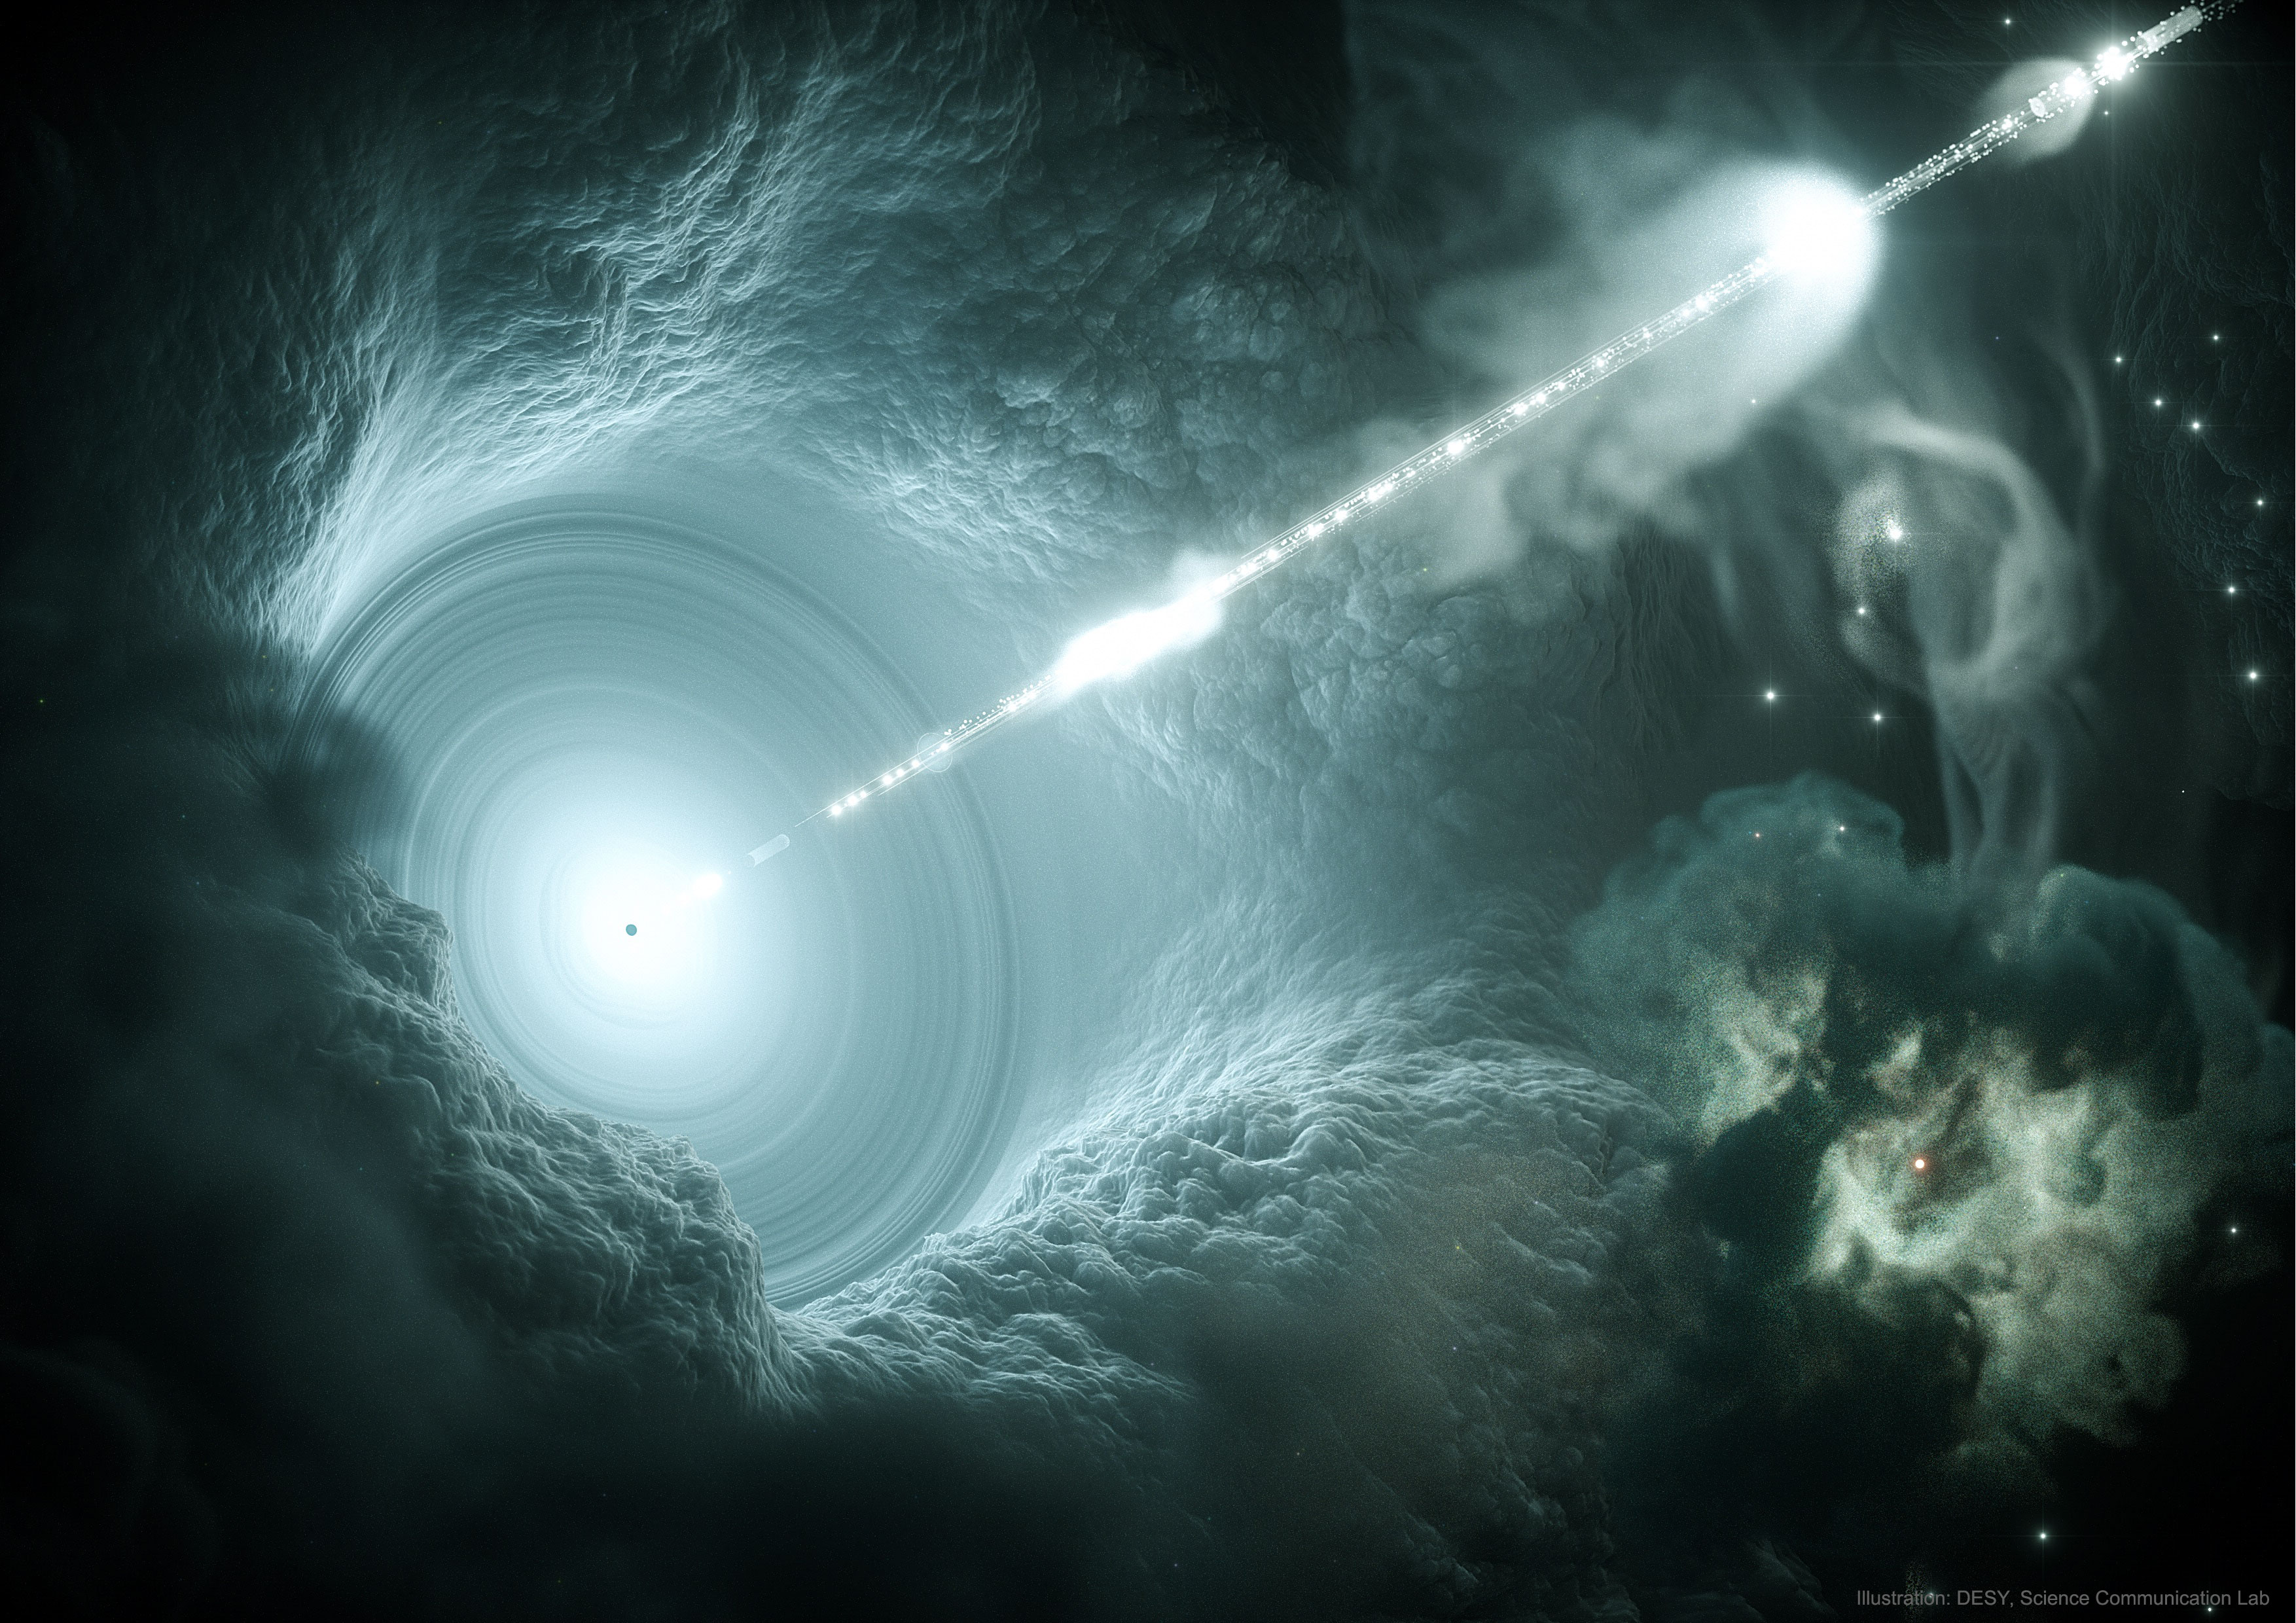
\includegraphics[width=0.49\textwidth]{chapter3/img/quazar.jpg}
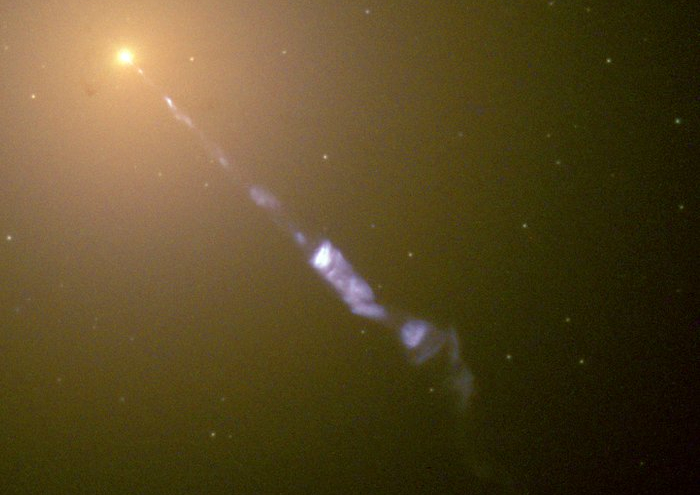
\includegraphics[width=0.49\textwidth]{chapter3/img/jet_crop.jpg}
\caption{Left: artist impression of a blazar which is recently been linked to a possible origin of extragalactic neutrinos \cite{TXS}. Illustration from DESY, Science Communication Lab. Right: Image from the Hubble telescope where we see a jet streaming out from the center of galaxy M87.}
\end{figure}

Charged partices have large cyclotron radii in AGNs and the relativistic jets could provide the necessary mechanisms to accelerate particles to ultra-high energies. Pierre Auger hinted to a correlation of the highest-energy cosmic rays with the positions of nearby active galactic nuclei \cite{Abraham:2007si}. Recently, a collaborative effort of IceCube, Fermi-LAT, MAGIC and others observed a coincidence of high-energy neutrinos and a blazar making them very good candidates of sources of extragalactic neutrinos \cite{IceCube:2018dnn}.

Misschien nog net iets meer uitwerken hoe UHECRs hier uit kunnen komen?
\subsubsection{Gamma Ray Bursts}
The most catastrophic deaths of massive stars or mergers of neutron-neutron stars or a neutron star and a black hole result into Gamma Ray Bursts (GRBs). GRBs are named after the burst of gamma rays that is followed by a longer-lived afterglow of electromagnetic radiation at longer wavelengths. These bursts are the most energetic explosions in the electromagnetic spectrum and occur when a high-mass star collapses to form a neutron star or black hole. A typical burst releases as much energy in a few seconds than the Sun will do in it's entire 10 billion-year lifetime and temporarily outshines the rest of the galaxy\footnote{GRBs were first discovered in the late 1960s by accident. The Vela sattelites had additional gamma ray detectors designed to detect very fast busts of gamma rays which are expected to be produced by nuclear tests in space \cite{Klebesadel:1973iq}}. GRBs are isotropically distributed, making them extragalactic in origin \cite{Meegan:1992xg}.

An often used model to explain how charged particles could reach extremely high energies is called the \textit{fireball model}. This internal-external shock model assumes that kinetic energy of an ultra-relativistic flow is dissipated in internal collisions. When the shock hits the surrounding matter it is slowed down and gives rise to the signature afterglow \cite{Piran:2004ba}. After initial the initial progenitor phase (see below) a plasma of photons, electrons, positrons and baryons develops into the formed jets. In this initial phase, the fireball is radiation-dominated and optically thick for photons, making it invisible in the electromagnetic spectrum. Due to radiative pressure the fireball expands at relativistic speeds ($\gamma$-factors $>$ 100) to the point that it becomes more and more transparent. If the central engine produces multiple shocks with different velocities there will be internal shocks, which give rise to the observed burst emission. In this mechanism, the ultra-relativistic matter can transfer it's kinetic energy to the acceleration of particles, explaining cosmic ray production. Later shocks of the jets with surrounding matter would explain the signature afterglow seen in GRBs.

Although there is still much ongoing discussion, GRBs are sometimes subdivided into two regions: \textit{long gamma ray bursts} ($t_{burst} > 2$s) and \textit{short gamma ray bursts} ($t_{burst} < 2s$). Long bursts originate from collapsars: a massive star core-collapse forms a black hole and surrounding matter is pulled into an accretion disk. Short burts hint to progenitors that are extremely compact, where neutron-neutron star or neutron star and black hole mergers are the most probable explanation. The recent detection of the gravitational waves can provide a significant contribution to the understanding of these sources \cite{TheLIGOScientific:2017qsa,Abbott:2017oio,Abbott:2017gyy,Abbott:2017vtc,Abbott:2016nmj}.

\begin{figure}
\centering
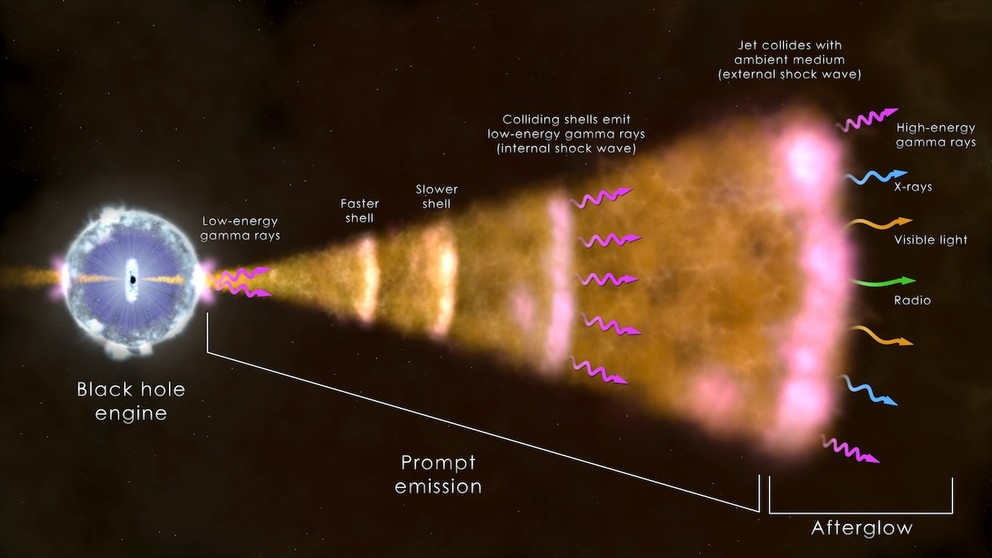
\includegraphics[width=0.6\textwidth]{chapter3/img/fireball.jpg}
\caption{In the fireball model ..... Image from NASA Goddard space flight center.}
\end{figure}

\subsubsection{Starburst galaxies}
Galaxies that undergo an episode of large-scale star formation, are called \textit{starburst galaxies}. Most of these are in the midst of a merger close encounter with another galaxy. Several experiments have shown their gamma ray emission at several hunderd GeV to be two to three orders of magnitude of that in our own Galaxy \cite{Acero:2009nb,Karlsson:2009hd}. Galactic scale winds from the central regions are possible sources for cosmic ray acceleration.

\subsubsection{Galaxy clusters}
When galaxies are bound togheter by gravity they are referred to as \textit{galaxy clusters}. They can contain around 100 to 1000 galaxies and have typical mass ranges around $10^{14}-10^{15}$ Solar masses. Through merging and accretion of dark matter and baryonic gas, galaxy clusters are expected to generate powerful shock waves on large scales. Shocks with significant velocities could provide the necessary conditions for cosmic ray acceleration \cite{•1538-4357-689-2-L105}.

\subsection{Propagation}
Doen of niet?

\section{Air showers}
\label{sec:airshowers}
When primary cosmic ray particles hit the Earth's atmosphere they give rise to a large shower of secondary particles. At low- to mid-energy ranges the abundance of cosmic rays is large enough for these showers to be analyzed with balloon or satellite experiments. As indicated in section \ref{subsec:whatarecosmicrays}, the flux of high-energy cosmic rays is so small, there is a need for very large-scale detectors, measuring kilometers in instrumented area.\\
\newline
The interaction length of nuclei with high energies is too small for them to be able to further than tens of kilometers in height. They will interact with an atmospheric nucleus and produce secondary particles. These particles, on their turn, decay or further interact with the atmosphere and give rise to an \textit{extensive air shower} if the production of new particles is large enough. Some of these particles will be stopped, but others are capable of reaching the Earth or even penetrate deep inside it. Although air showers are of significant importance in cosmic ray studies, we will only give a brief summary of the most noteworthy features and it's main importance for this analysis.
An air shower has three components: the hadronic, muonic and electromagnetic. The hadronic component can be seen as the core of the shower consisting of high-energy hadrons. The interactions and subsequent decays of these hadrons fuel the electromagnetic and muonic parts. A schematic overview is given in Figure \ref{fig:airshower}. If the primary particle is a photon the shower is made up almost exclusively of an electromagnetic component. Because the lateral size of an electromagnetic cascade is caused by multiple scattering of electrons and positrons the lateral size of these showers is relatively small (radius around 1 km for a transversely downgoing 100 TeV photon). In hadronic cascades, on the other hand, the lateral size is caused by the transverse momenta of the secondary particles making these showers much larger (radius arond 4km for a transversely downgoing 100 TeV proton) \cite{Grupen:2005rx}.

\begin{figure}
\centering
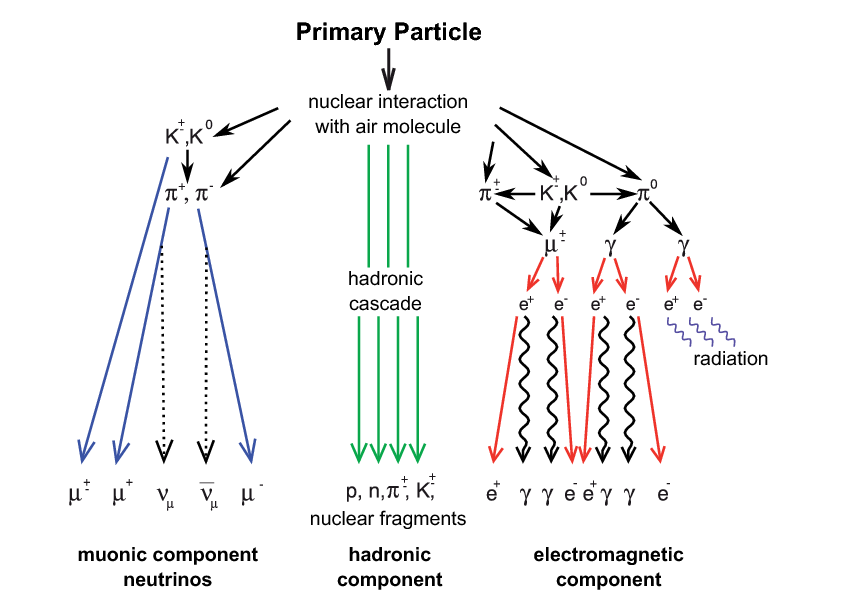
\includegraphics[width=0.8\textwidth]{chapter3/img/airshower.png}
\caption{Schematic view of an extensive air shower with a clear distinction between the three components. Image from KASKADE collaboration.}
\label{fig:airshower}
\end{figure} 

\subsection{Hadronic component}
When a proton interacts with a nucleus it interacts with a proton or neutron and will most often produce charged or neutral pions
\begin{equation}
\begin{split}
p+N &\rightarrow p+N + k\pi^+ + k\pi^- +r\pi^0,\\
p+N &\rightarrow n+N + (k+1)\pi^+ + k\pi^- + r\pi^0,\\
\end{split}
\end{equation}
where $N$ stands for a nucleon of an atmospheric nucleus and $k$ and $r$ are the multiplicities of the produced pions. The example for heavier nuclei from this is straightforward. On average, one-third of the hadron production will be neutral pions which decay immediately into electromagnetic particles 

\begin{alignat}{2}
\pi^0 &\rightarrow \gamma  +\gamma \\ &&(98.8\%) \textrm{ or}\\
\pi^0 &\rightarrow e^+ + e^- + \gamma \\ &&(1.17\%).
\end{alignat}
The other two-thirds will be charged particles and have a lot longer lifetime, making them much more probable to interact with air nuclei. After having traveled a distance corresponding to their mean interaction length, charged particles interact again with air nuclei if their energy is great enough. 90\% of these charged particles are new pions and 10\% of the daughter particles are kaons. Pions almost exclusively decay into muons ($\pi^+ \rightarrow \mu^+ + \nu_{\mu}$) and the most dominant kaon decay modes are (similar for $K^-$) \cite{pdg}

\begin{alignat}{2}
K^+ &\rightarrow \pi^+ + \pi^0  &&(20.7\%),\\
K^+ &\rightarrow \mu^+ + \nu_{\mu}  &&(63.6\%),\\
K^+ &\rightarrow \pi^0 + e^+ + \nu_e  &&(5\%),\\
K^+ &\rightarrow \pi^0 + \mu^+ + \nu_{\mu}  \ \ &&(3.4\%),\\
\end{alignat} 
where the first decay mode fuels the hadronic component further. The remaining decay modes enter in the EM and muonic components. The total number of hadrons reaching sea level is very small and when they do, they are immediately stopped.

\subsection{Muonic component}
Muons are the dominant component of particles reaching sea level (around 80\%). Most muons which are produced in an EAS are able to reach so far due to their relativistic velocities and lifetime of 2.2 $\mu$s\footnote{The half-survival length of 5 GeV muons is $L = \ln(2) \times \gamma \times 2.2 \mu\textrm{s} \times 0.9998 \times c = \gamma \times 456$ m $\approx 23$ km. The relativistic time dilation is of crucial importance here!}. They have relatively low ionization losses compared to electrons, making them very penetrating and are therefore referred to as the \textit{hard component}. Muons can also decay and contribute to the electromagnetic compionent via

\begin{equation}
\begin{split}
\mu^+ &\rightarrow e^+ + \nu_e + \bar{\nu}_\mu, \\
\mu^- &\rightarrow e^- + \bar{\nu}_e + \nu_\mu.
\end{split}
\end{equation}

\subsection{Electromagnetic component}
At each hadronic interaction, slightly more than a third of the energy goes into the electromagnetic component. Since most hadrons re-interact, eventually most of the primary energy finds its way into the electromagnetic component. Muons can produce \textit{delta electrons} or electron-positron pairs from pair production (see section???).

At energies above a few MeV photons interact with matter via pair production and convert into an electron-positron pair. High-energy electrons and positrons primarily emit photons via bremsstrahlung. These two processes are repeated until the photons fall below the pair production threshold and bremsstrahlung energy loss starts to dominate. Because electrons lose their energy fast they are almost immediately stopped when they reach dense matter (Earth's surface) and hence referred to as the \textit{soft component}.
\subsection{Neutrino component}
Leeg laten en pas beschrijven hieronder?



\section{Neutrinos}
\label{sec:neutrinos}
As by-products of cosmic ray collisions with matter, neutrinos provide incontrovertible evidence for hadronic acceleration. Since these particle are weakly-interacting they can escape much denser environments and hold crucial information about the origins of their production environments. Because these particles barely interact, their detection is difficult. Similarly to cosmic rays, neutrinos cover a broad range in energy (see Figure \ref{fig:neutrinorange}), calling for different types of detector to cover this large spectrum. 

\begin{figure}[t]
\centering
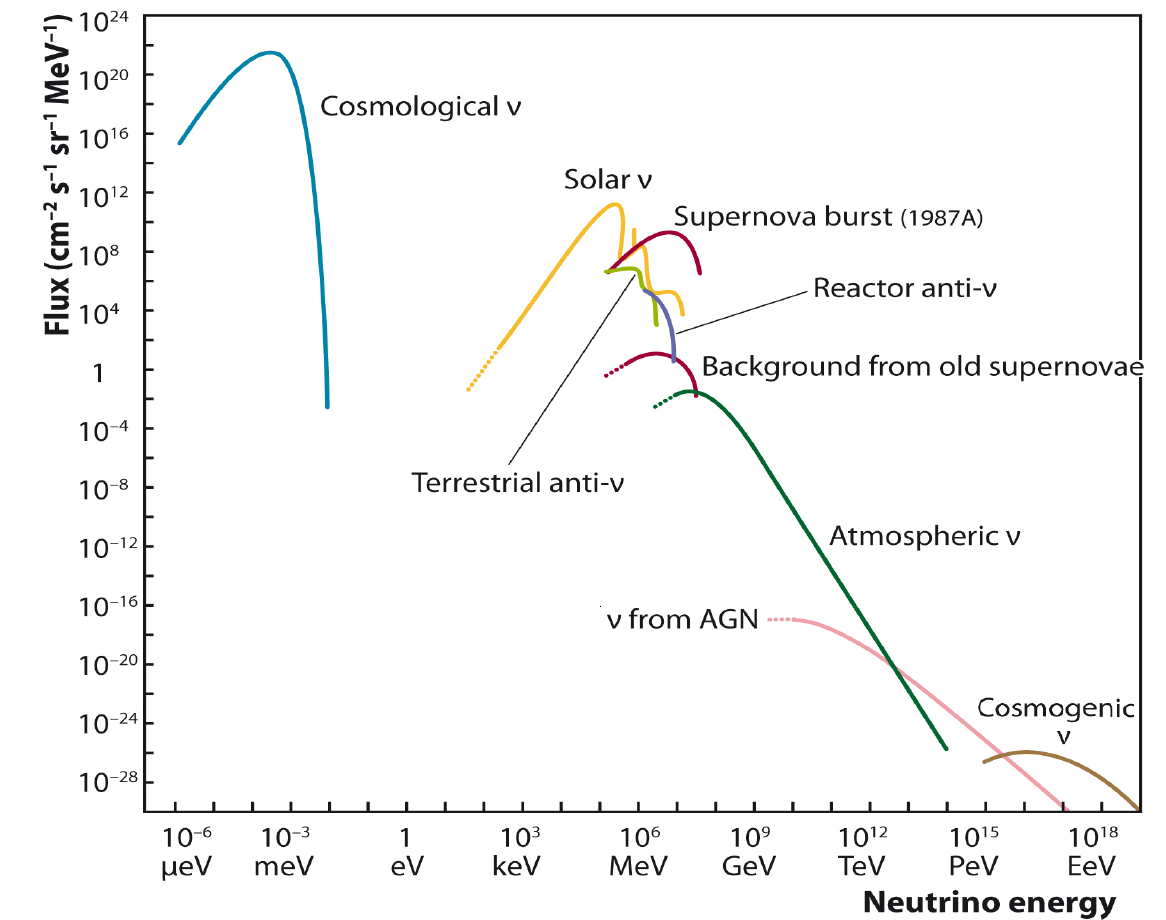
\includegraphics[width=0.7\textwidth]{chapter3/img/neutrinospectrum.png}
\caption{Plot illustrating several neutrino fluxes which cover a huge range of energy. Illustration from \cite{Katz:2011ke}.}
\label{fig:neutrinospectrumall}
\end{figure}

Cosmic rays are deflected in inter- and extragalactic magnetic fields and therefore their arrival direction at Earth does not hold much pointing information (Figure \ref{fig:sourceinfo}, left). Light ranging from radio to gamma rays on the electromagnetic spectrum is of a crucial importance in astrophysics but has it's limitations. Photons can be absorbed by interstellar medium, or are trapped in opaque sources. At higher energies ($\approx 10^{14}$ eV) photons interact and produce electron-positron pair ($\gamma + \gamma \rightarrow e^+ + e^-$). Unless the sources are closeby no photons are capable of reaching Earth (see Figure \ref{fig:sourceinfo}, right). Neutrinos escape from the sources more easily and are not deflected by magnetic fields making them key messengers in identifying cosmic ray accelerators. In the following we will go over the different types of neutrinos which are detectable on Earth.

\begin{figure}[t]
\centering
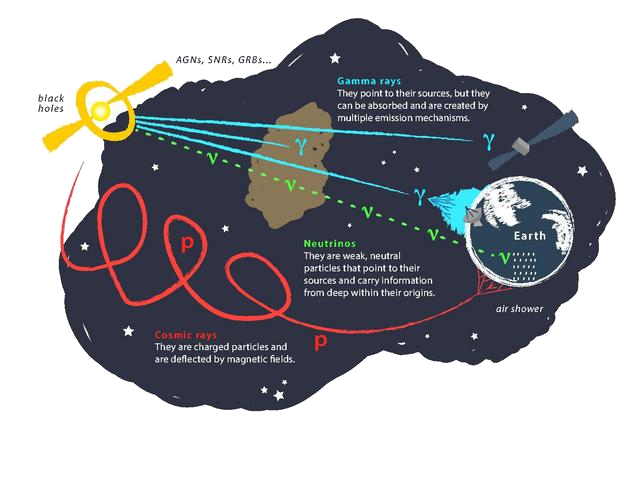
\includegraphics[width=0.4\textwidth]{chapter3/img/sourceinformation_3.jpg}
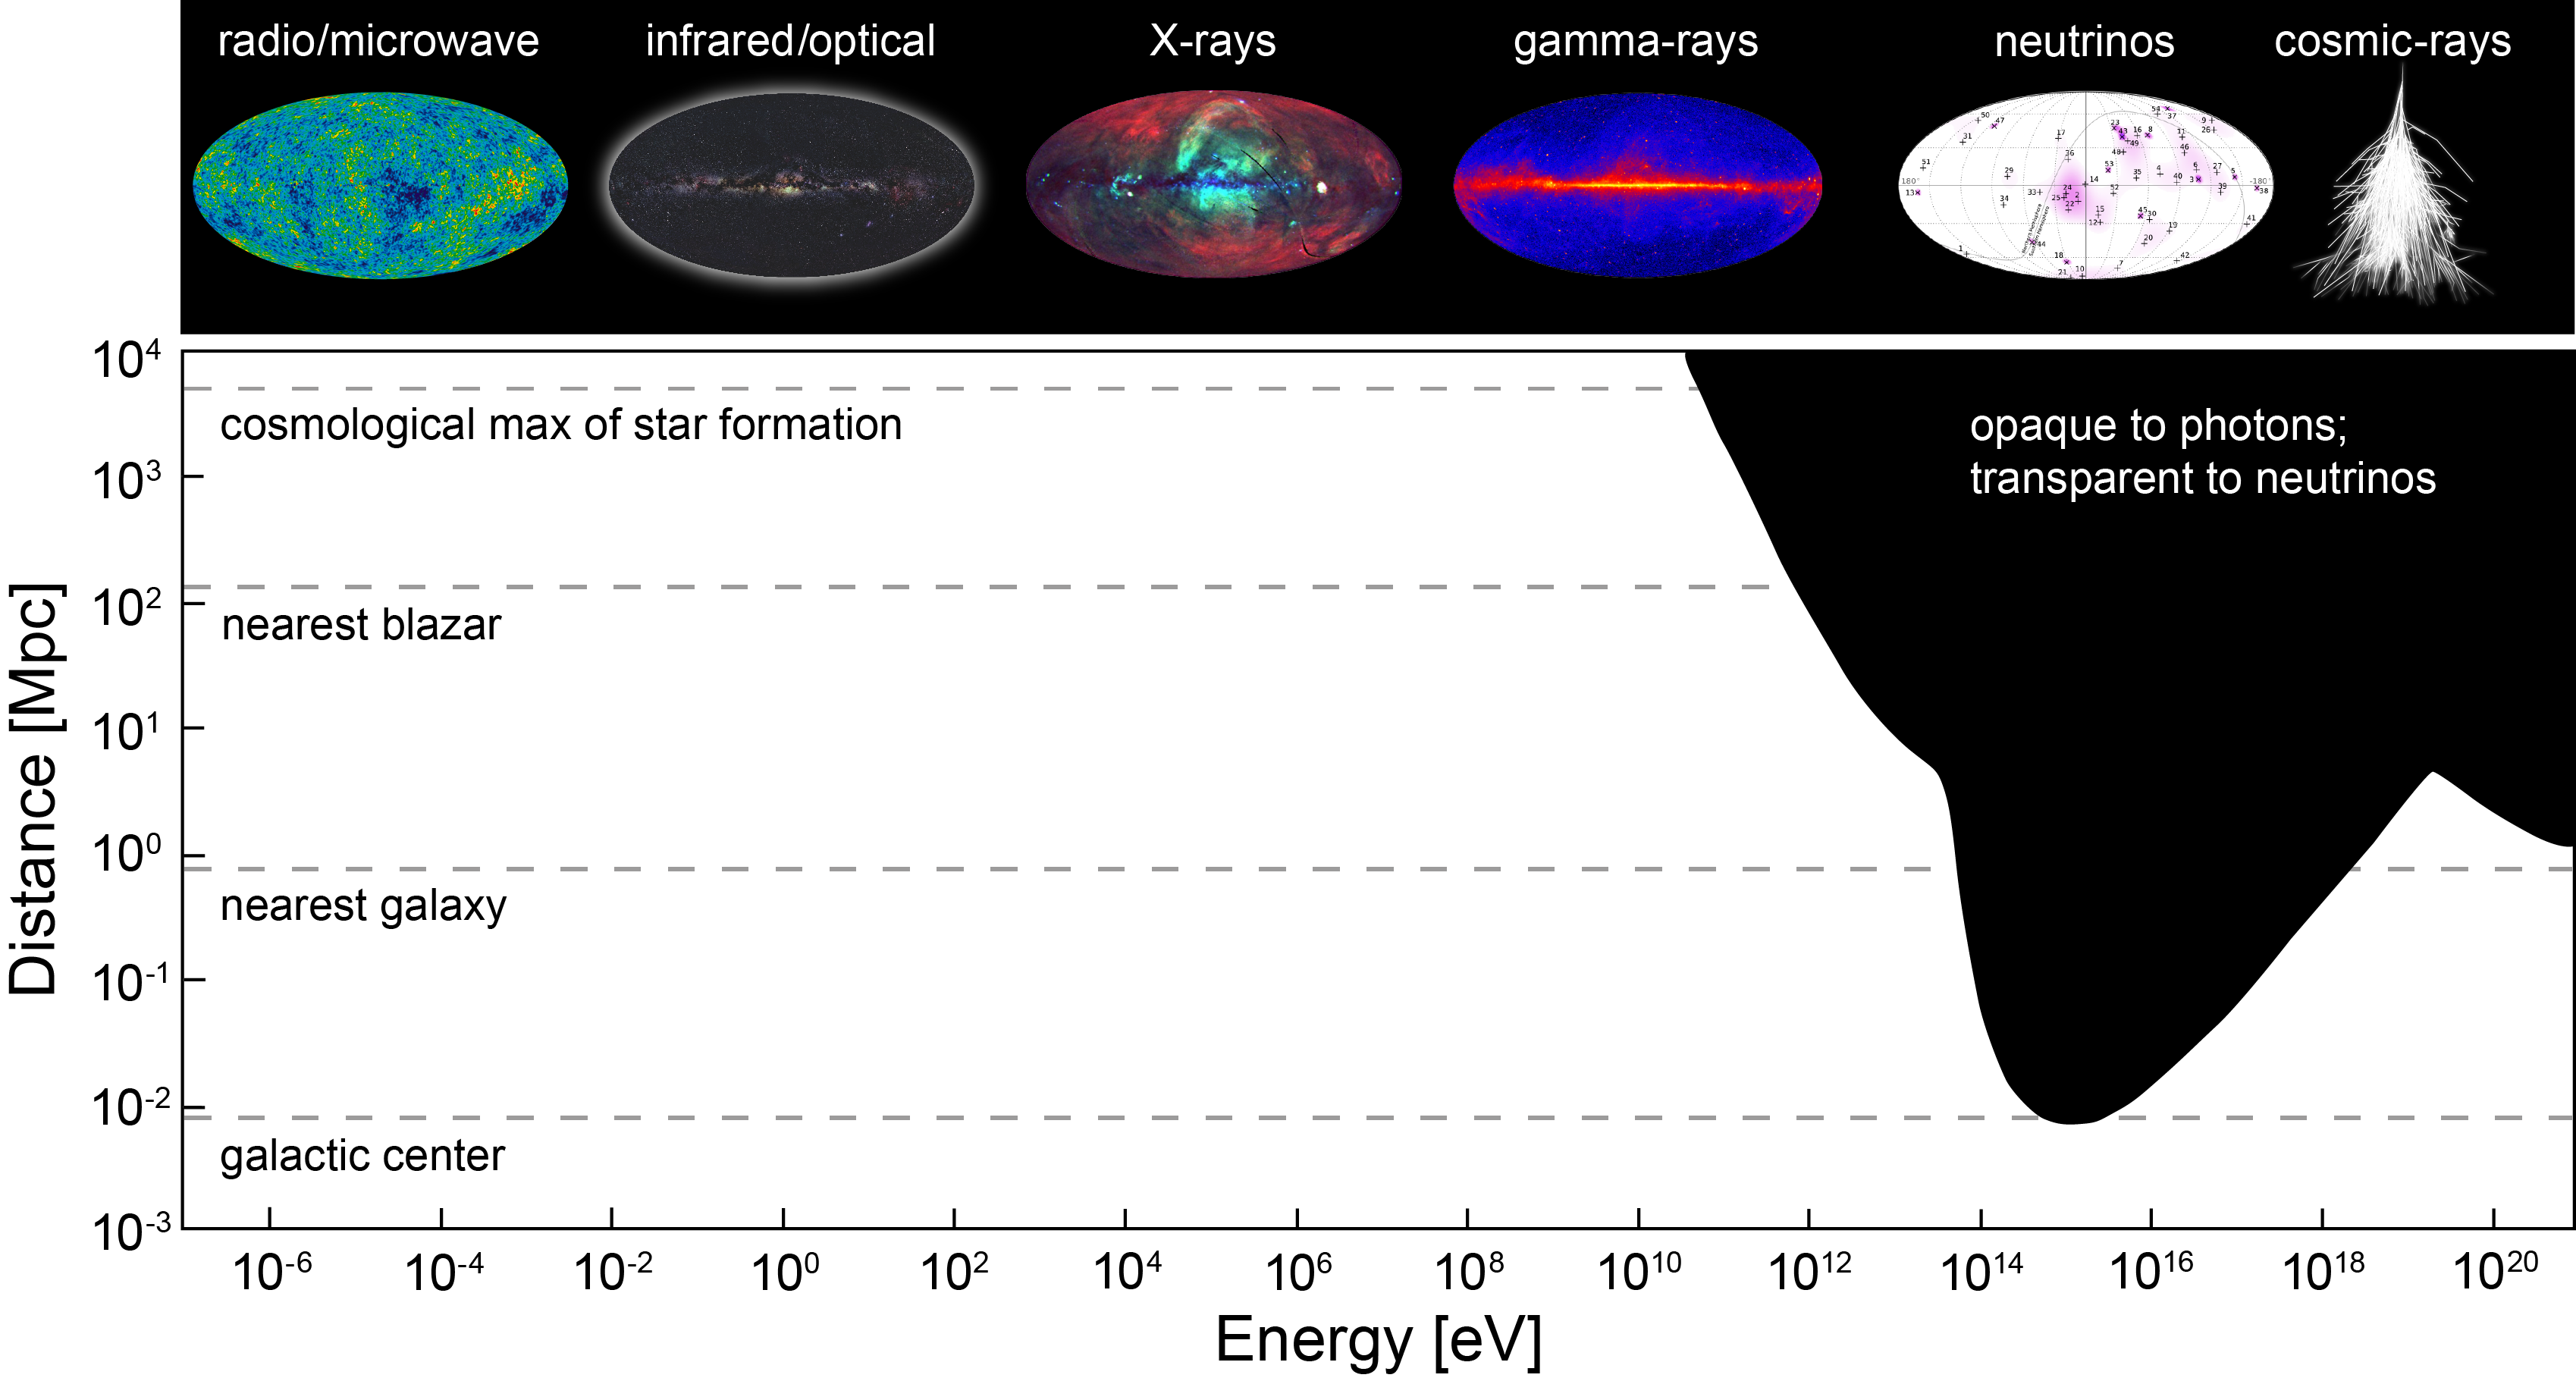
\includegraphics[width=0.59\textwidth]{chapter3/img/opaque-to-photons.png}
\caption{Left: Artist impression of the path that several types of particles travel before reaching Earth. Right: Illustration of the visibility of sources in function of their distance and the photon energy. The signature dip in the photon visibility comes from the pair production peak when photons interact with the CMB. Both illustrations from the IceCube collaboration.}
\label{fig:sourceinfo}
\end{figure}


\subsection{Conventional}
Neutrinos are produced in large abundances in air showers as explained in \ref{sec:airshowers}. The neutrinos that are produced with low to high energies ($\approx$ MeV to PeV range) are called \textit{atmospheric} or \textit{conventional} neutrinos. They are primarily produced in pion on kaon decay. Due to helicity effects, pion and kaon decay to electron(s) (neutrinos) is strongly suppressed compared to decays into muon(s) (neutrinos). As a result, the ratio of electron neutrinos to muon neutrinos is a factor of around two

\begin{equation}
\frac{N\left( \nu_\mu + \bar{\nu}_\mu\right) }{N\left(\nu_e + \bar{\nu}_e\right)} \approx 2,
\end{equation}
which should be clear when we look at the example of pion decay where the muon decays as well

\begin{align}
\pi^+ &\rightarrow \mu^+ + \nu_\mu \\
& \rightarrow e^+ + \nu_e + \bar{\nu}_\mu + \nu_\mu.
\end{align}
The most referred to calculations for the atmospherical neutrino flux was done by Honda et al. \cite{Honda:2006qj}.
\begin{figure}[t]
\centering
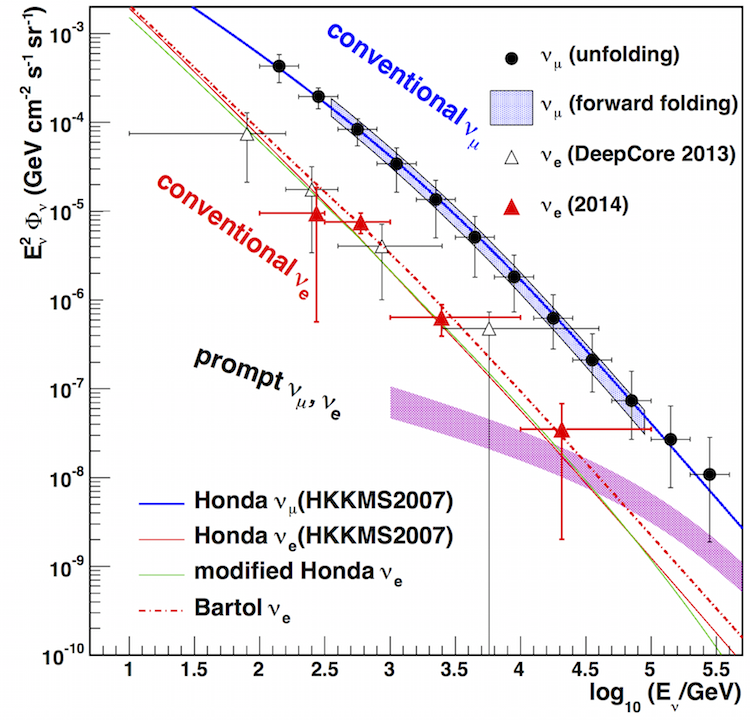
\includegraphics[width=0.39\textwidth]{chapter3/img/neutrinospectrum2.png}
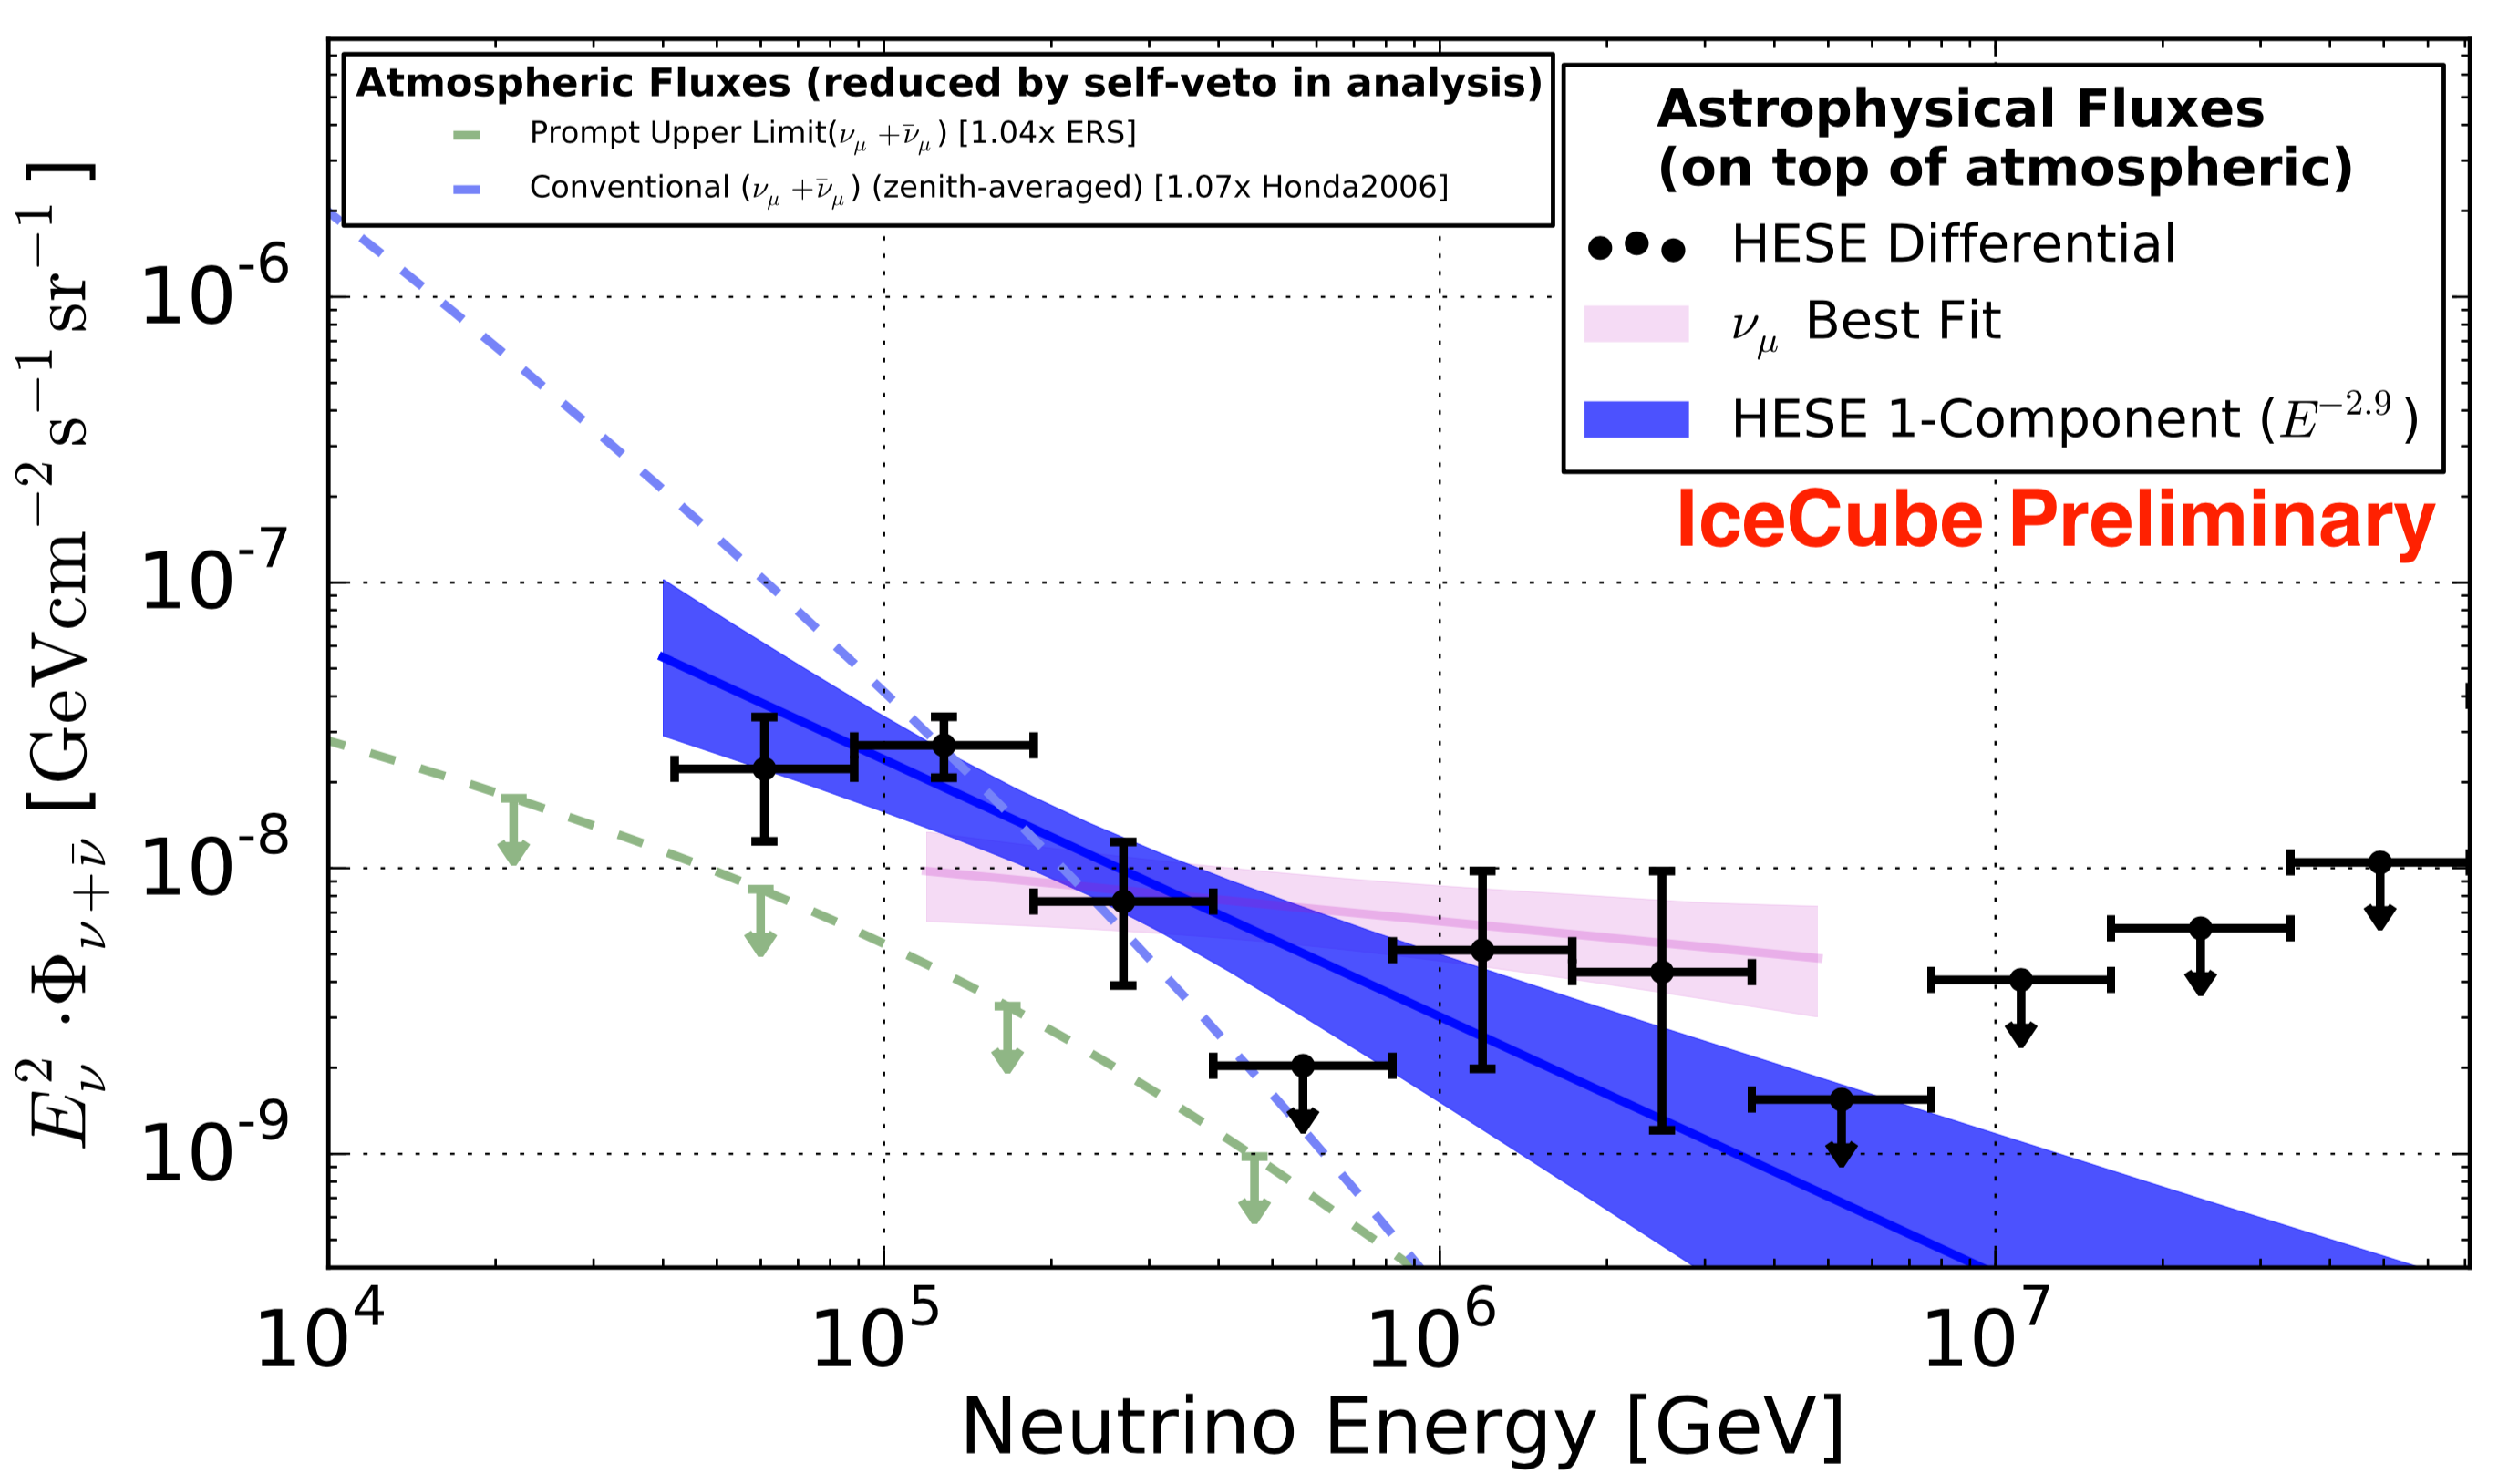
\includegraphics[width=0.6\textwidth]{chapter3/img/astroflux.png}
\caption{Left: Measurement from the IceCube collaboration showing the difference in $\nu_e$ and $\nu_\mu$ flux. Right: Measured differential astrophysical flux using contained events (points) and a fit do that data (blue line and band), compared with the best fit obtained from throug-going $\nu_\mu$ (pink line and band). From Ref. \cite{Aartsen:2017mau}}.
\label{fig:neutrinospectrum2}
\end{figure}

\subsection{Prompt}
Charmed mesons, also called D mesons, are the lightest particles that contain charm quarks\footnote{$D^0: c\bar{u}, \bar{D}^0: u\bar{c}, D^+: c\bar{d}, D^-: d\bar{c}$}. Hints of charm particles were first seen in cosmic rays in 1971 by Niu et al. \cite{doi:10.1143/PTP.46.1644}. The production of these particles is strongly suppressed, but are expected to exhibit a harder spectrum than conventional neutrinos do. These mesons have short lifetimes (hence the name: prompt) and decay into netrinos independent of their energy and arrival direction. Therefore, their energy spectrum is expected to follow that of primary cosmic rays. Their contribution at higher energies can be non-negligible or even become dominant. To this date is has not been possible to observe this prompt component, but remains an interesting signal in diffuse neutrino searches and could contribute significantly to background expectations.  The most referred to calculations for the prompt neutrino flux was done by Endberg et al. \cite{Enberg:2008te}.
\subsection{Astrophysical}
\label{subsec:astro}
Astrophysical neutrinos are expected to be created when cosmic rays interact close to their interaction sites. Because they are neutral and are unlikely to be absorbed, astrophysical neutrinos are expected to reveal more information about these sources. To first order, these neutrinos would follow the spectrum of cosmic rays at their production. As indicated in section \ref{para:power}, this is equal to an $E^{-2}$ powerlaw spectrum from Fermi shock acceleration. The majority of these neutrinos are expected to arise from decays from pions which were created in these cosmic-ray interactions ($\pi \rightarrow \mu + \nu_\mu$) followed by the muon decay ($\mu \rightarrow e + \nu_e + \nu_\mu$). The resulting flavor ratio fraction is $\nu_e: \nu_\mu: \nu_\tau = 1:2:0$ at the source. Neutrino oscillations across cosmological distances give an expected $\nu_e: \nu_\mu: \nu_\tau = 1:1:1$ expectation at Earth. As can be seen in Figure \cite{fig:neutrinospectrum2}.

The spectrum is expected to follow the hardest spectrum of the three and therefore dominates at the highest energies.

\subsection{Other neutrino sources}
\subsubsection{Cosmological}
Similar to the photons from the CMB, neutrinos would have been able to decouple from matter only seconds after the Big Bang. Due to the expansion of the universe, the temperature of the neutrinos has dropped to $\approx 1.95K$ due to redshift. At these energies direct detection is near to impossible. They have no measureable effect in large-scale neutrino detectors.
 
Mooie uitleg van redshift: https://www.forbes.com/sites/startswithabang/2016/09/09/cosmic-neutrinos-detected-confirming-the-big-bangs-last-great-prediction/
\subsubsection{Solar}
Nuclear fusion in the Sun is responsible for the production of electron neutrinos and is the largest contribution of neutrinos which can be detected on Earth. 86\% of neutrinos are produced by the proton-proton reaction

\begin{equation}
p + p \rightarrow d + e^+ + \nu_e.
\end{equation}
The remaining part is produced by reactions which involve more heavy particles. Having energies $<$ 20 MeV these neutrinos have no measurable effect in neutrino telescopes.
\subsubsection{Terrestrial neutrinos}
Radioactive decays from $\ce{^{40}K}$, $\ce{^{232}Th}$ and $\ce{^{238}U}$ account for almost all geoneutrinos. The reactions give rise to neutrinos from beta decay \cite{Wan:2016nhe}

\begin{alignat}{2}
\ce{^{40}_{19}K} + e^- &\rightarrow \ce{^{40}_{18}Ar} + \nu_e \ \ &&+1.505 \textrm{ MeV,}\\
\ce{^{40}_{19}K} &\rightarrow \ce{^{40}_{20}Ca} +e^- + \bar{\nu}_e \ \ &&+1.311 \textrm{ MeV,}\\
\ce{^{232}_{90}Th} &\rightarrow \ce{^{208}_{82}Pb} +6\alpha + 4e^- +4\bar{\nu}_e\ \ &&+42.652 \textrm{ MeV,} \\
\ce{^{235}_{92}U} &\rightarrow \ce{^{207}_{82}Pb} + 7\alpha + 4e^- + 4\bar{\nu}_e \ \ &&+46.402 \textrm{ MeV,}\\
\ce{^{238}_{92}U} &\rightarrow \ce{^{206}_{82}Pb} +8\alpha +6e^- + 6\bar{\nu}e \ \ &&+51.698 \textrm{ MeV.}
\end{alignat}
The maximal energies of these neutrinos are again too low to give a contribution to neutrino telescopes.
\subsubsection{Reactor neutrinos}
Nuclear reactors harnass energy from the splitting (fission) of heavy nuclei into lighter fission products. These neutron-rich daughter particles undergo beta decays ($n \rightarrow p+e^-+\bar{\nu}_e$). Reactor neutrinos are therefore always antineutrinos. The energy spectrum reaches a maximum around 10 MeV, making them again invisible for neutrino telescopes. 

\subsubsection{Supernova neutrinos}
The core collapse of stars where electrons and protons are compressed into neutrons as described in ??? dissipates most of it's energy in the production of neutrinos ($e^- + p^+ \rightarrow n + \nu_e$) \cite{Scholberg:2012id}. Depending on the distance of the source to the detector supernovae are only visible in a collective raise of the dark noise of the apparture \cite{Kopke:2011xb}.
\section{Cosmic ray and neutrino detectors}
\label{sec:detectors}

Heel kort: pg 5 Gaisser boek. Zo IC introduceren.

VERITAS, HESS, MAGIC, HAWC, PA, TA, Super-K, Antares, IceCube

Ook dat plotje waarbij je toont dat neutrinos interessanter zijn in hoge E omdat fotonen onzichtbaar worden!

The IceCube Collaboration instead tested the principle using neutrinos. Neutrinos interact with matter through the weak force — one of the four fundamental forces of nature. The influence of the weak force is limited to minute distances. As a result, interactions between neutrinos and matter are extremely improbable, and a neutrino can easily traverse the entire Earth unimpeded. This poses a challenge for physicists trying to study these elusive particles, because almost every neutrino will simply pass through any detector completely unnoticed.




In neutral-current reactions neutrinos lose energy, but are not absorbed

hier tot pg 50?